\begin{center}
    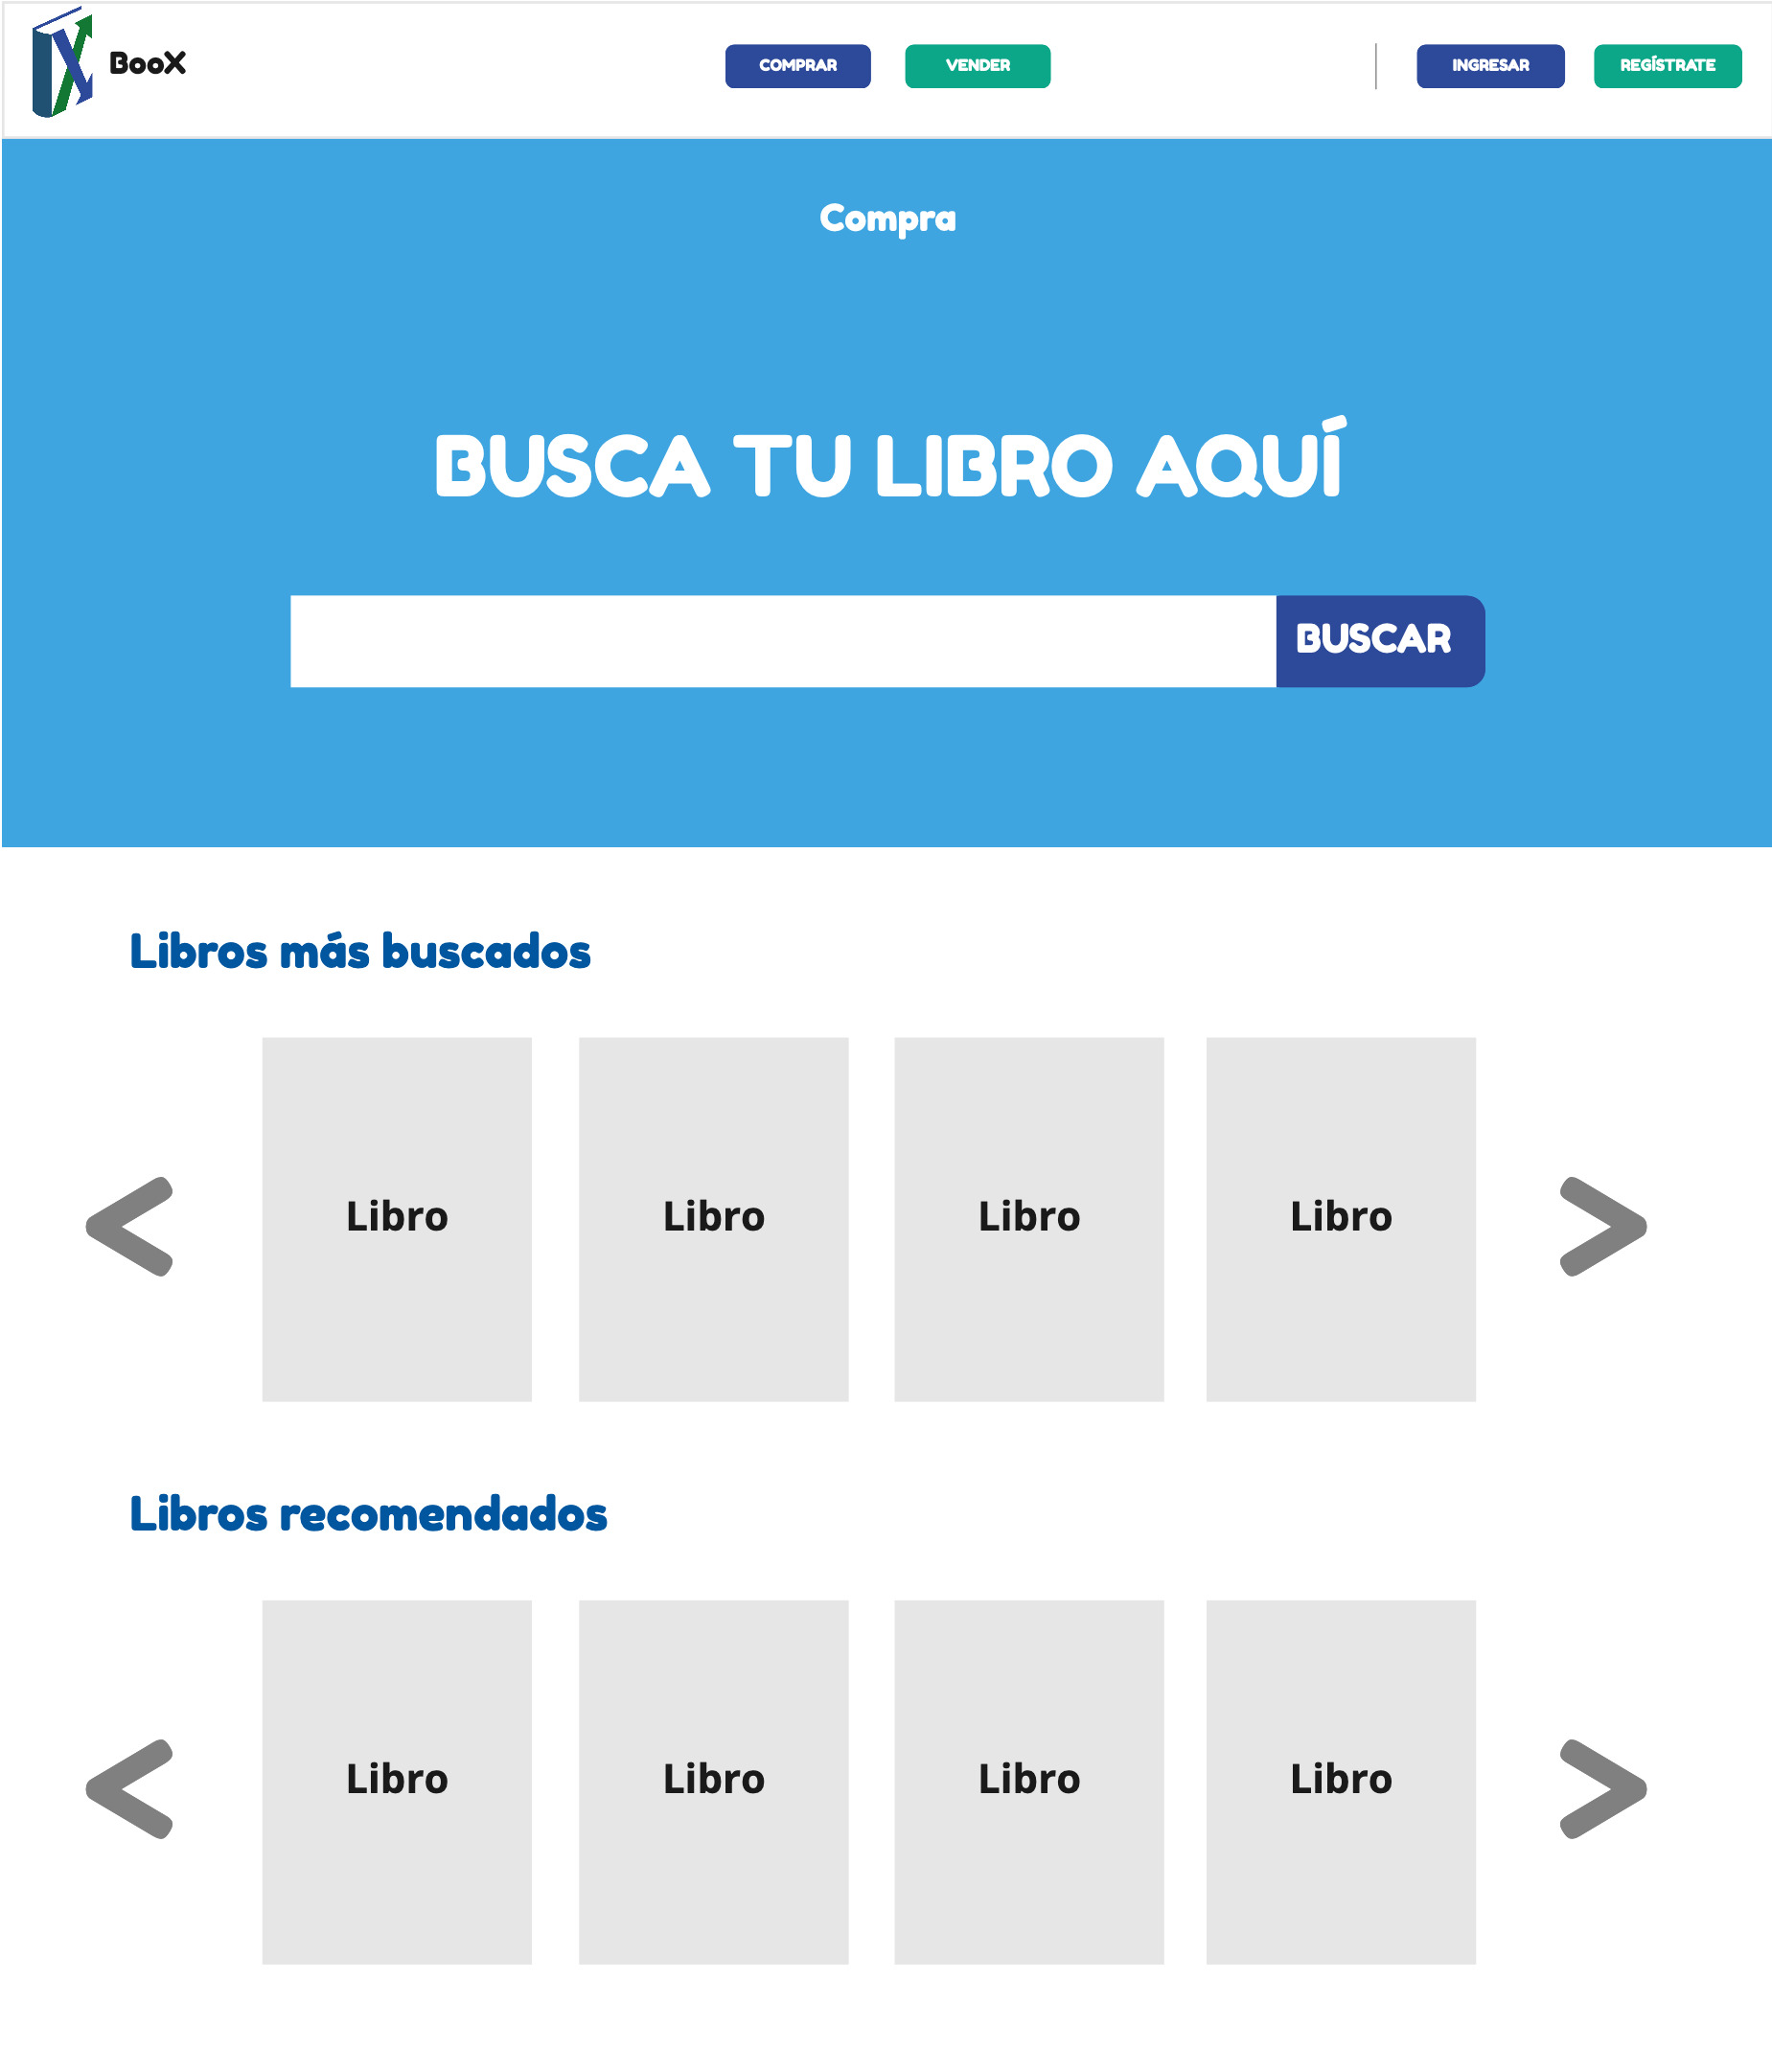
\includegraphics[width=300pt]{img/mockups/Huascar Retrieval Team - Landing.jpg}
\end{center}

User enters BooX and is redirected to the landing page. Here, the main action is the search bar, where the user can search books by title, ISBN or author. Below, book suggestions \footnote{Book suggestions are based on previous user actions. Thus, the user needs to have an account and log in to access this feature.} and trending books in a Netflix-style carousel.\\
\begin{center}
    \includegraphics[width=300pt]{img/mockups/Huascar Retrieval Team - Búsqueda.jpg}
\end{center}

Users can do a search and access it description and trending books without having to log in. However, an account is required to contact the seller and sell a book. To log in, the user clicks on the upper right corner. If the user does not have an account, he or she can click at the register button next to the log in or click in "create one" at the login page.\\
\begin{center}
    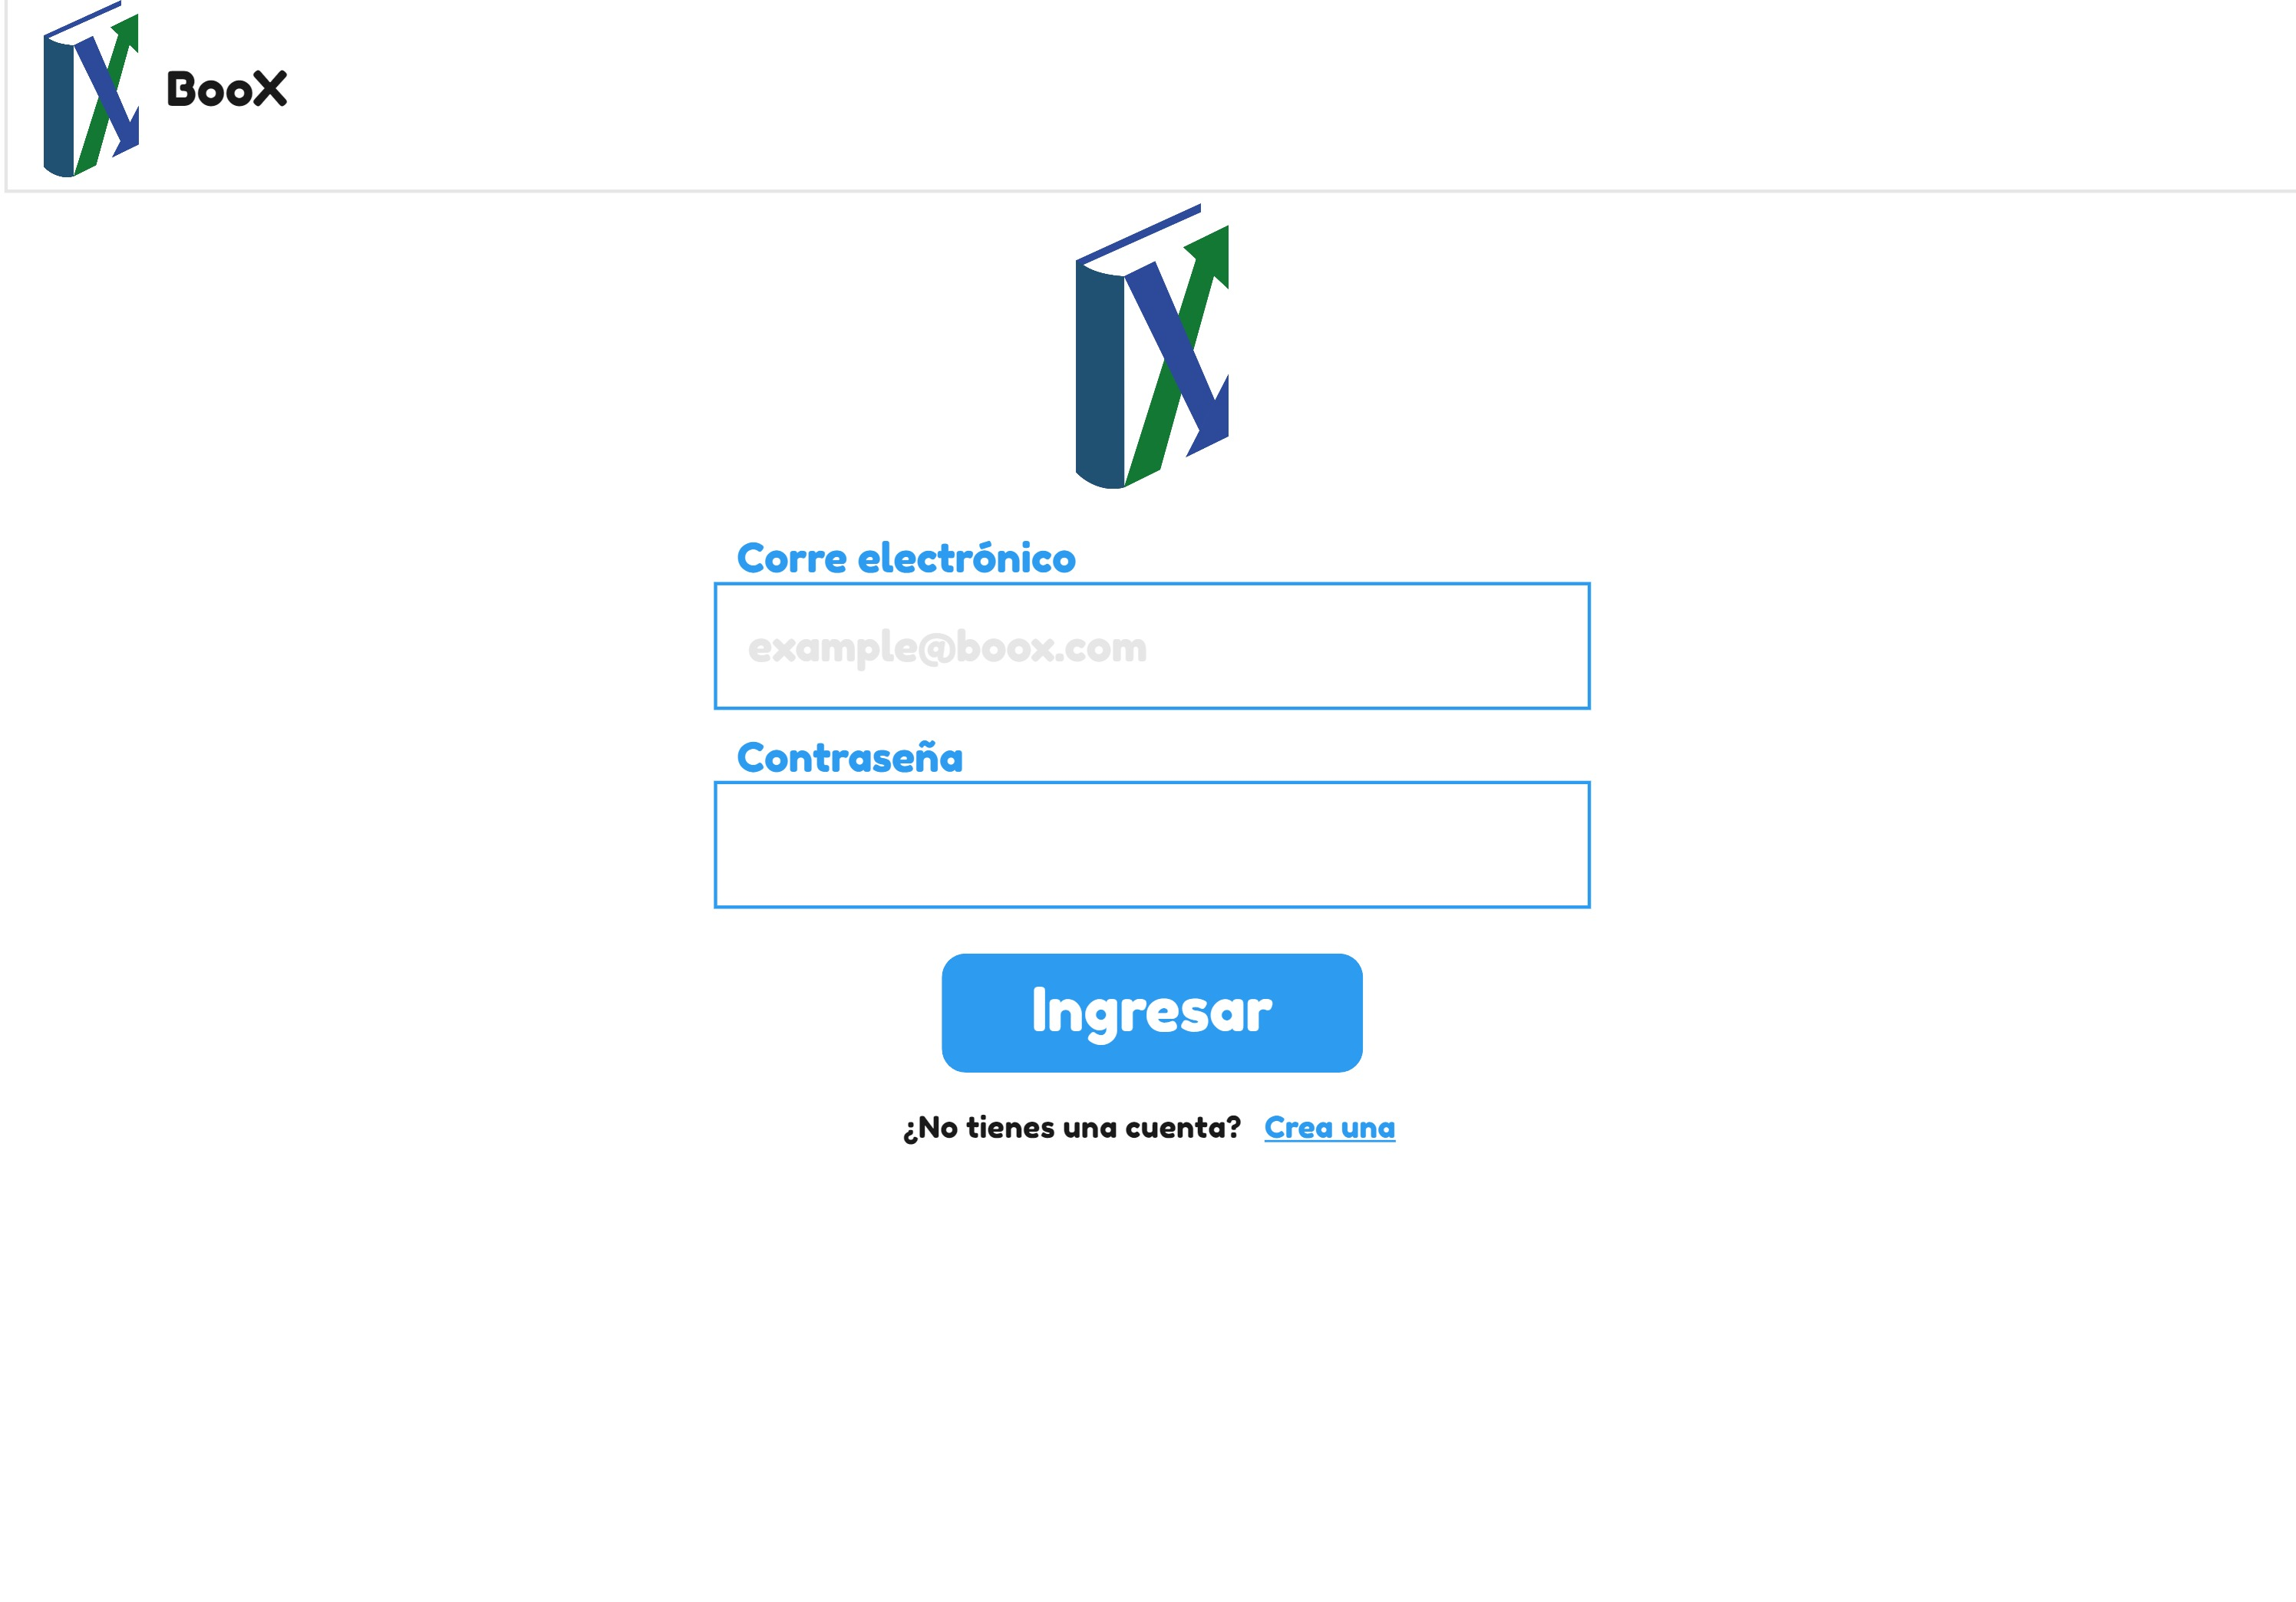
\includegraphics[width=300pt]{img/mockups/Huascar Retrieval Team - Login.jpg}
    \end{center}
    \subsubsection*{}
    \begin{center}
    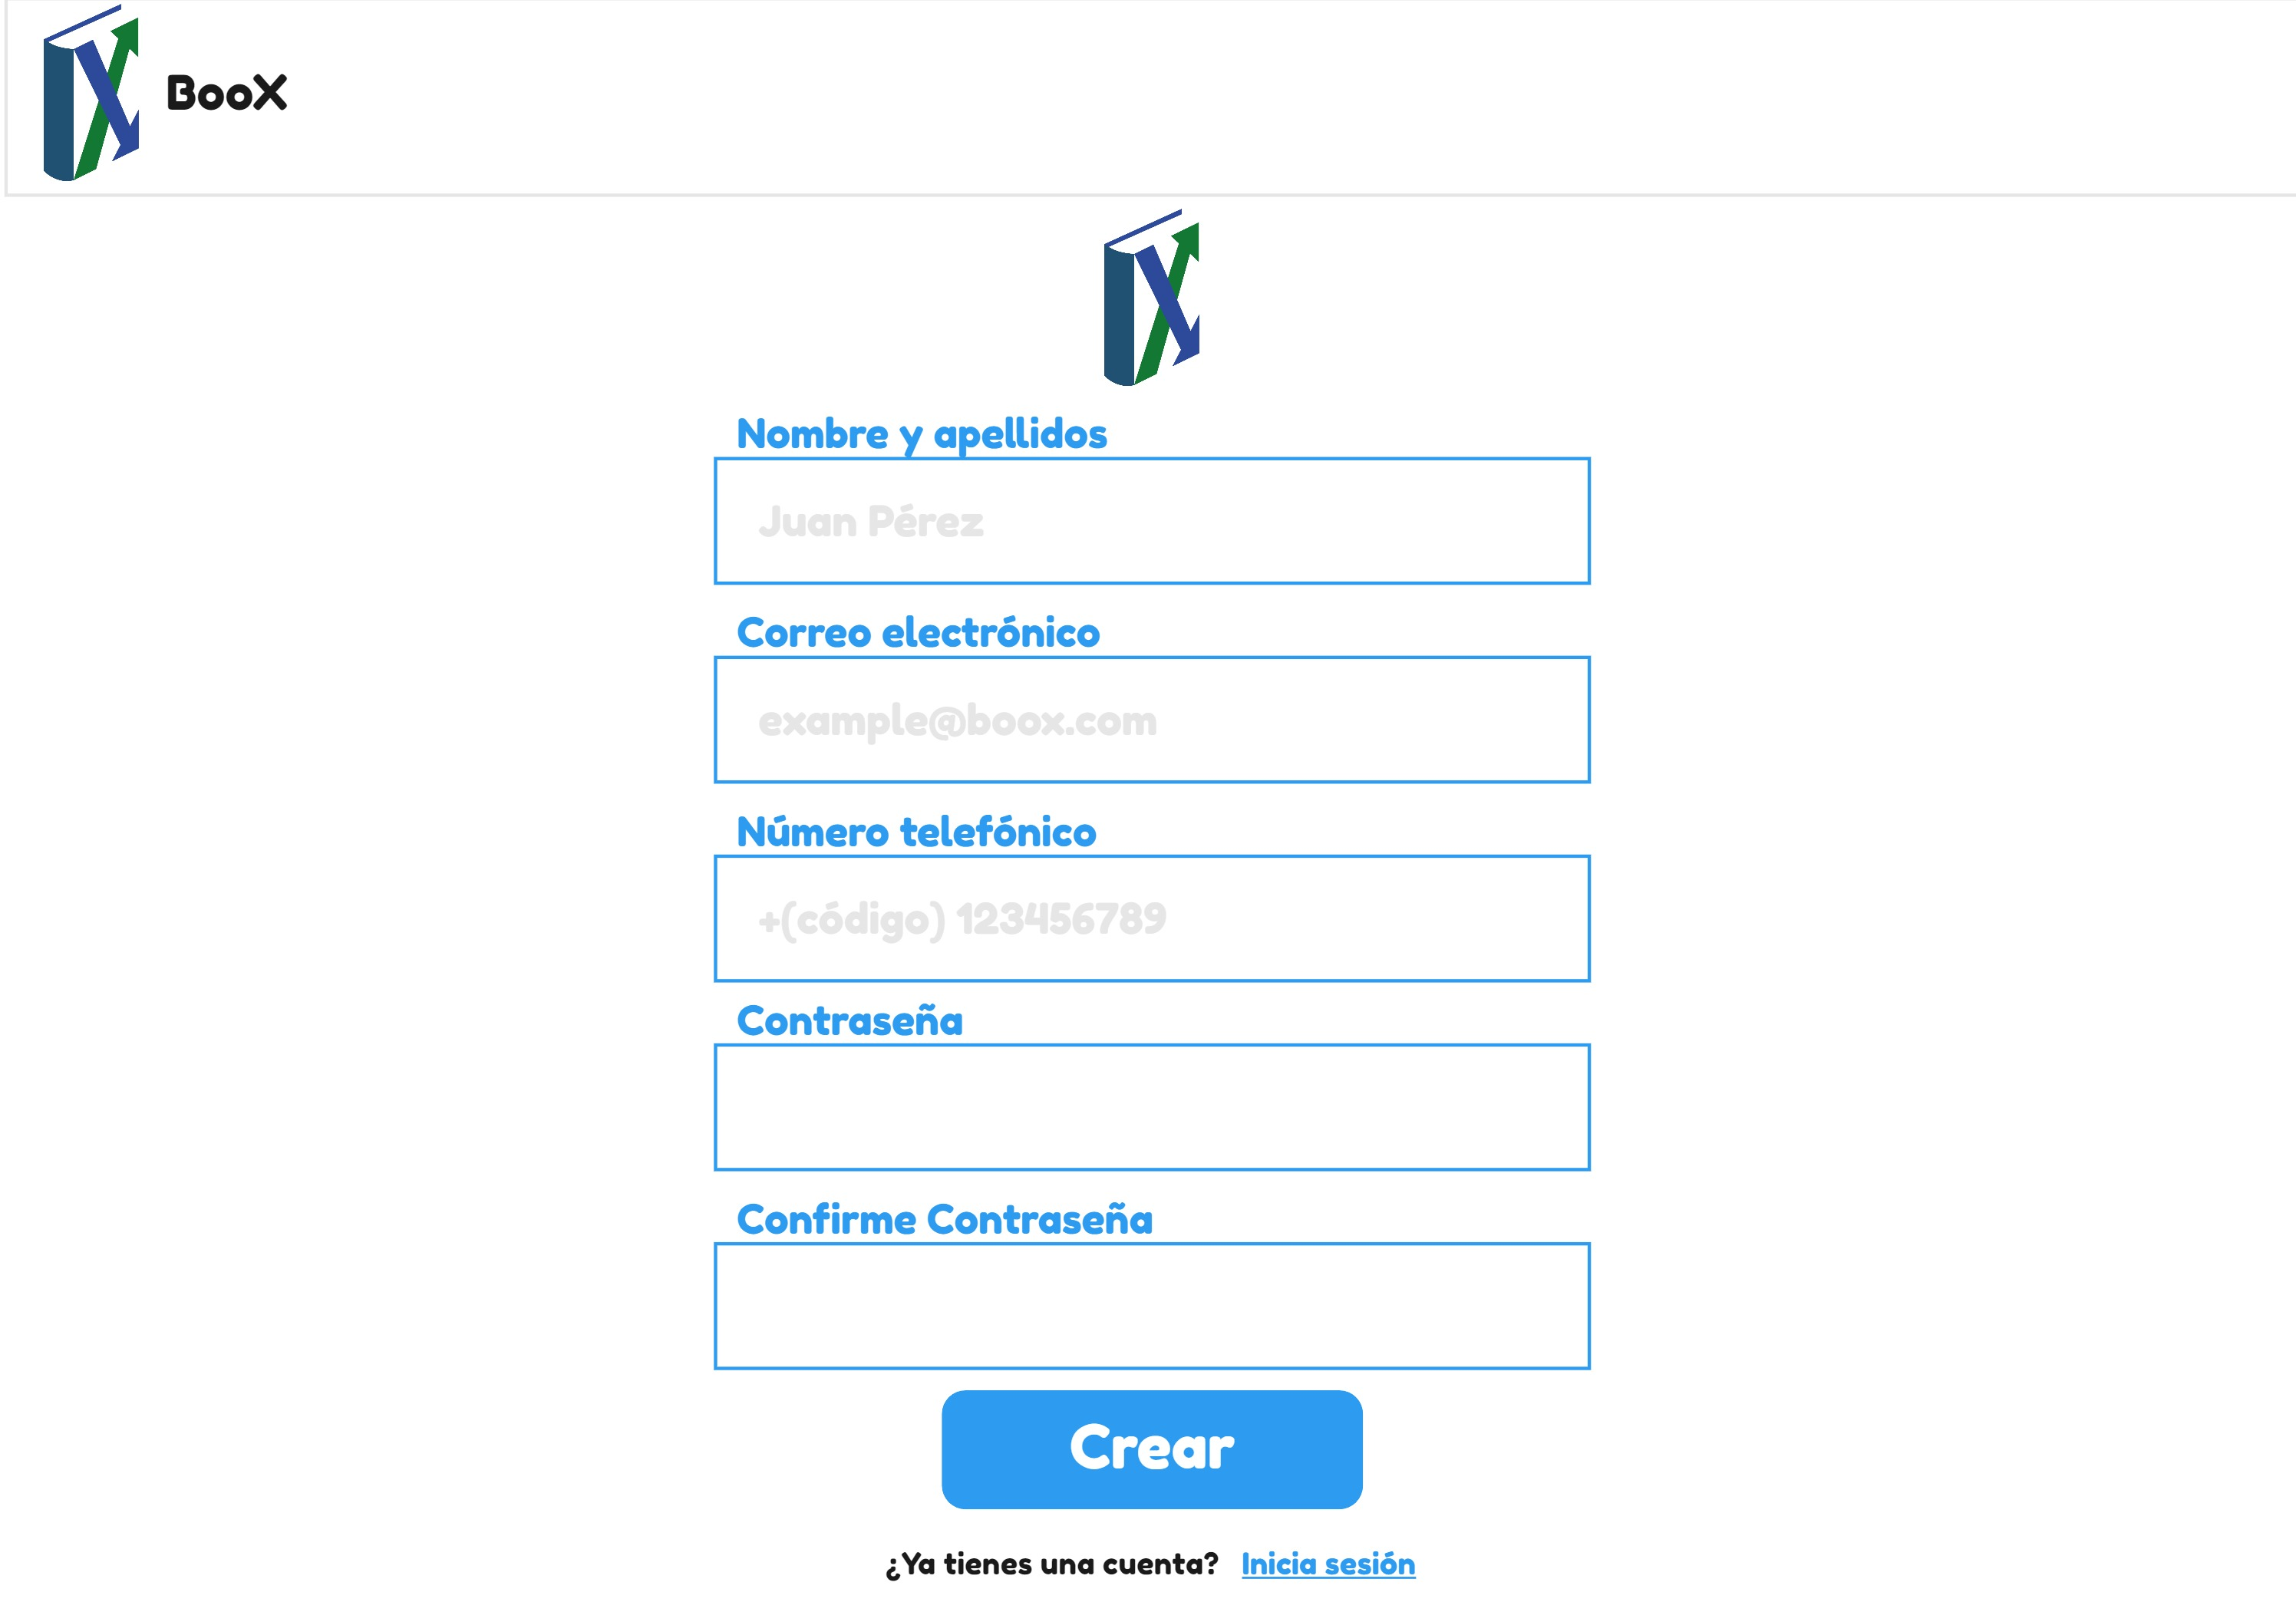
\includegraphics[width=300pt]{img/mockups/Huascar Retrieval Team - Registro.jpg}
\end{center}


After a search, a list of books is displayed. Each book contains details about itself  and its seller. For an advance search, a sidebar with options as the book conditions, genre and seller location is presented.\\

\begin{center}
    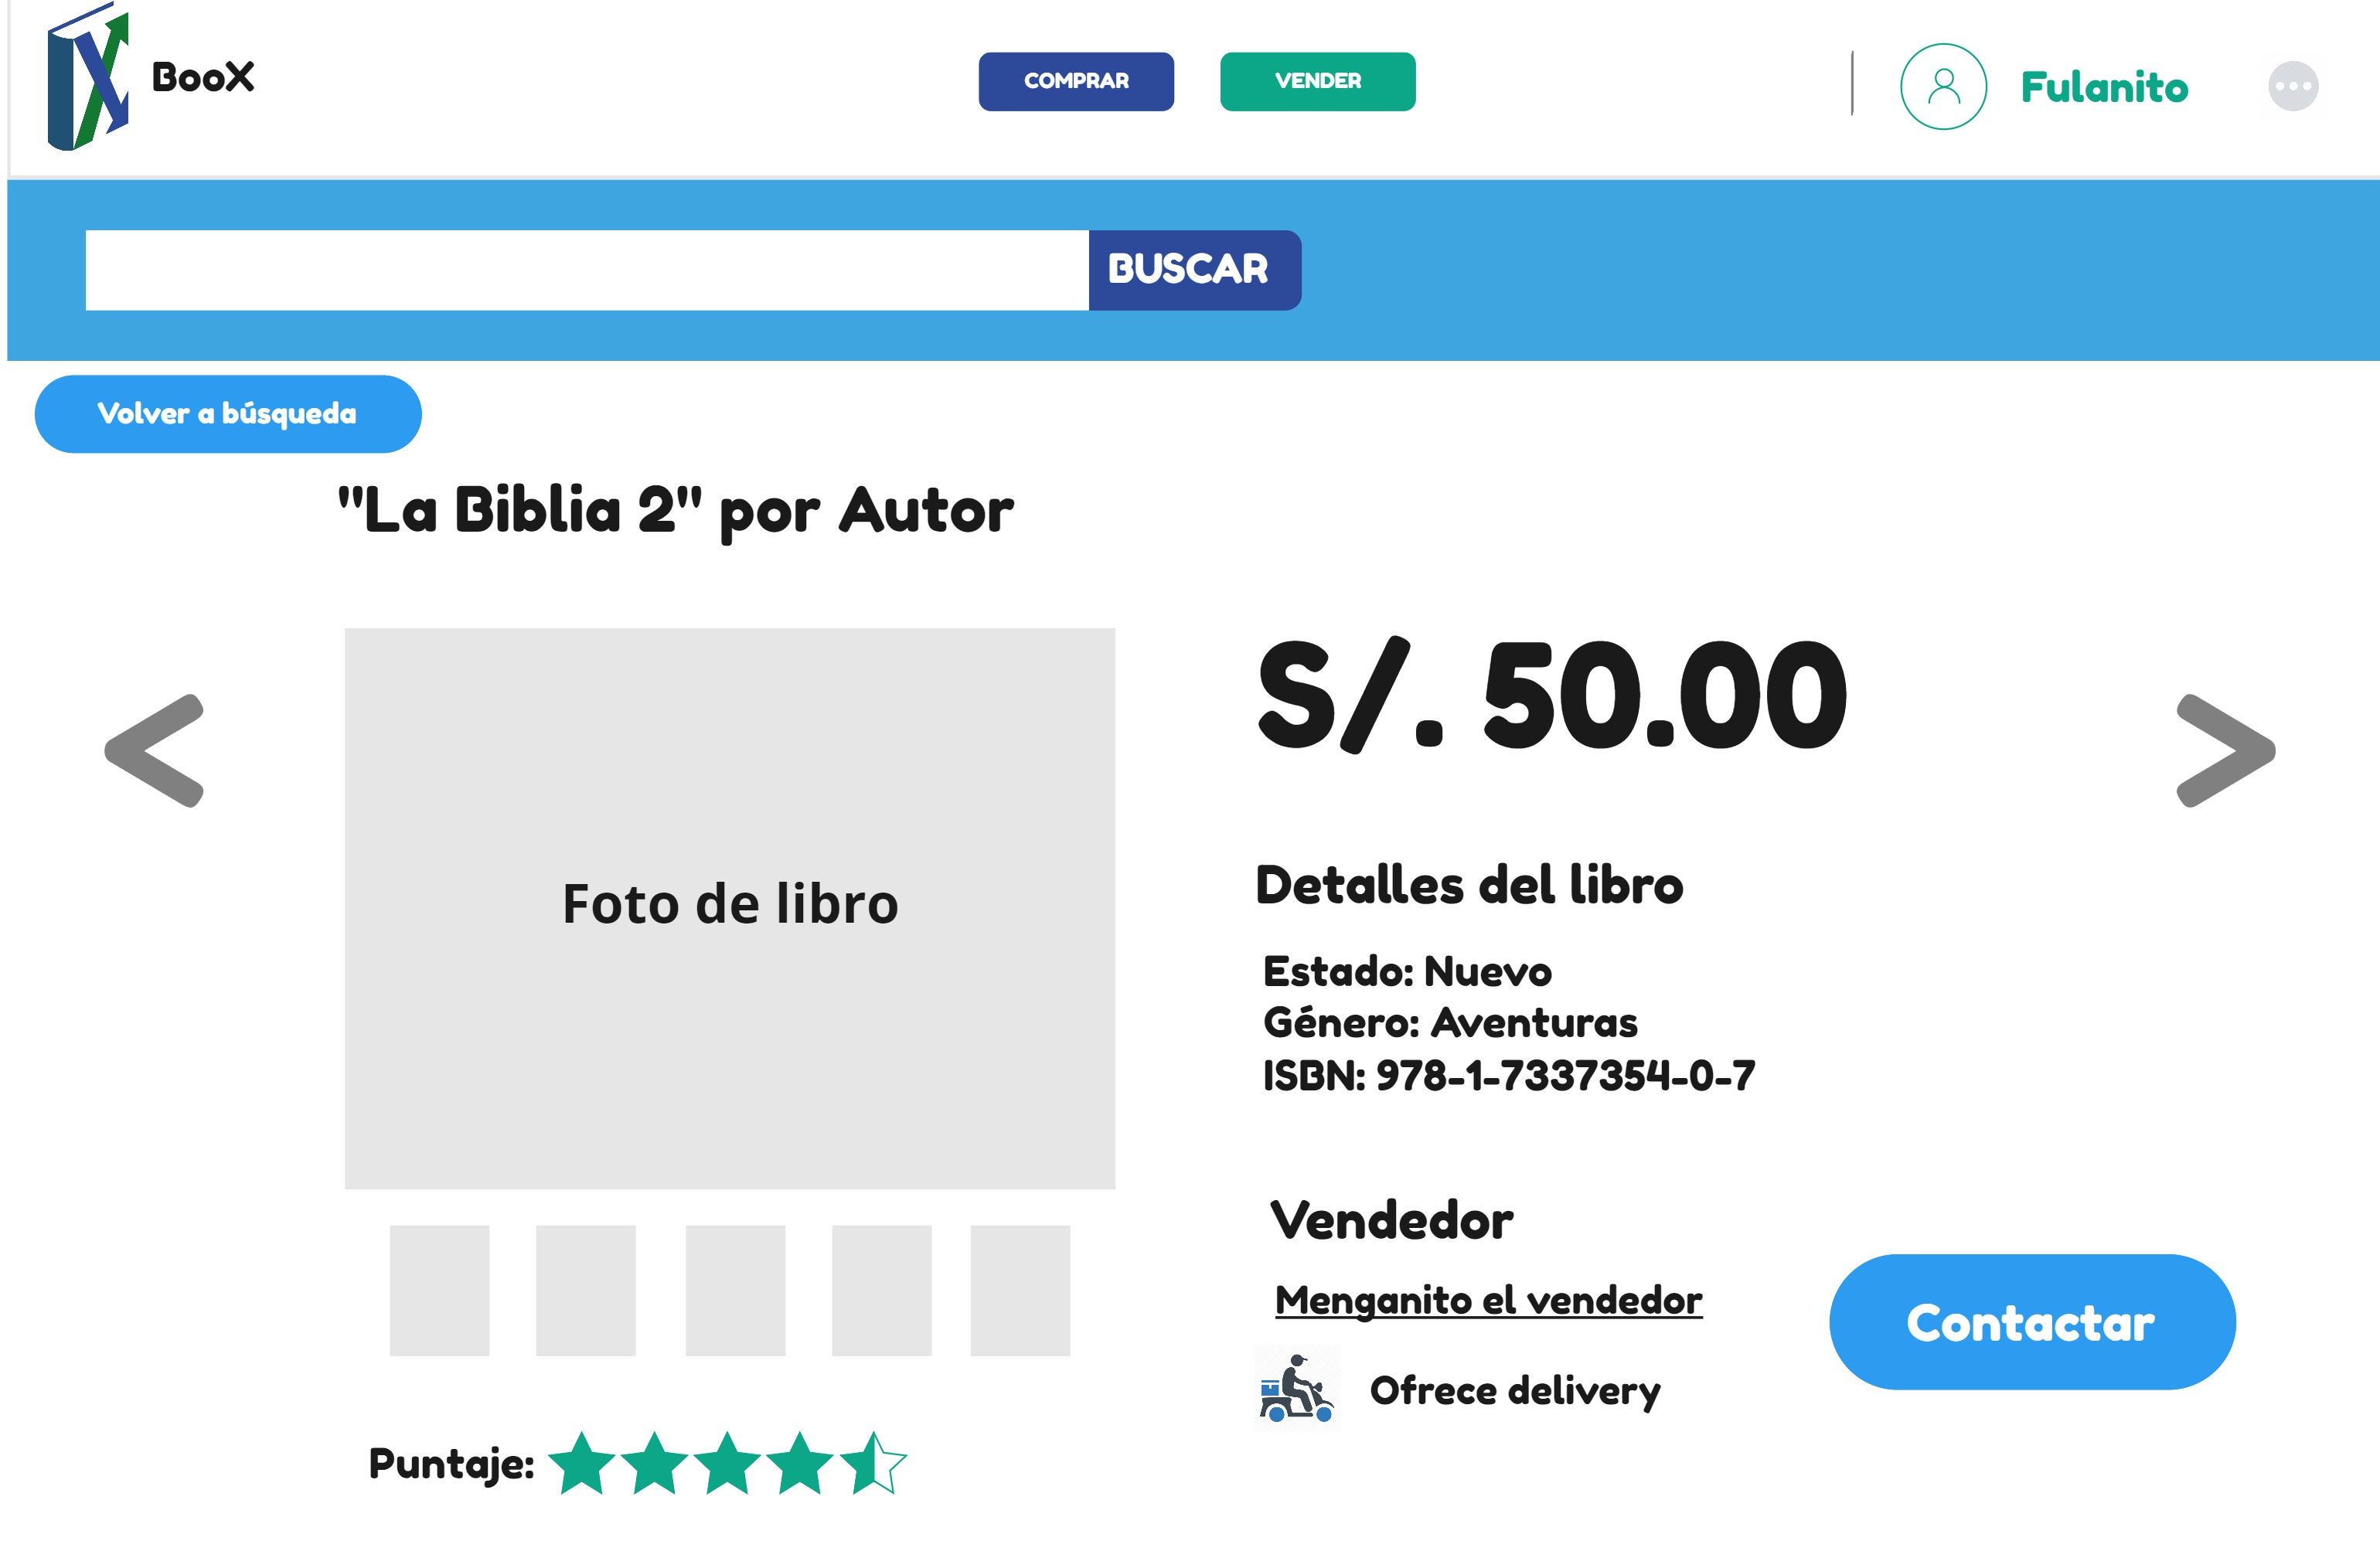
\includegraphics[width=300pt]{img/mockups/Huascar Retrieval Team - Detalles de libro.jpg}
\end{center}

When the user selects a book, the next page is displayed.\\
\begin{center}
    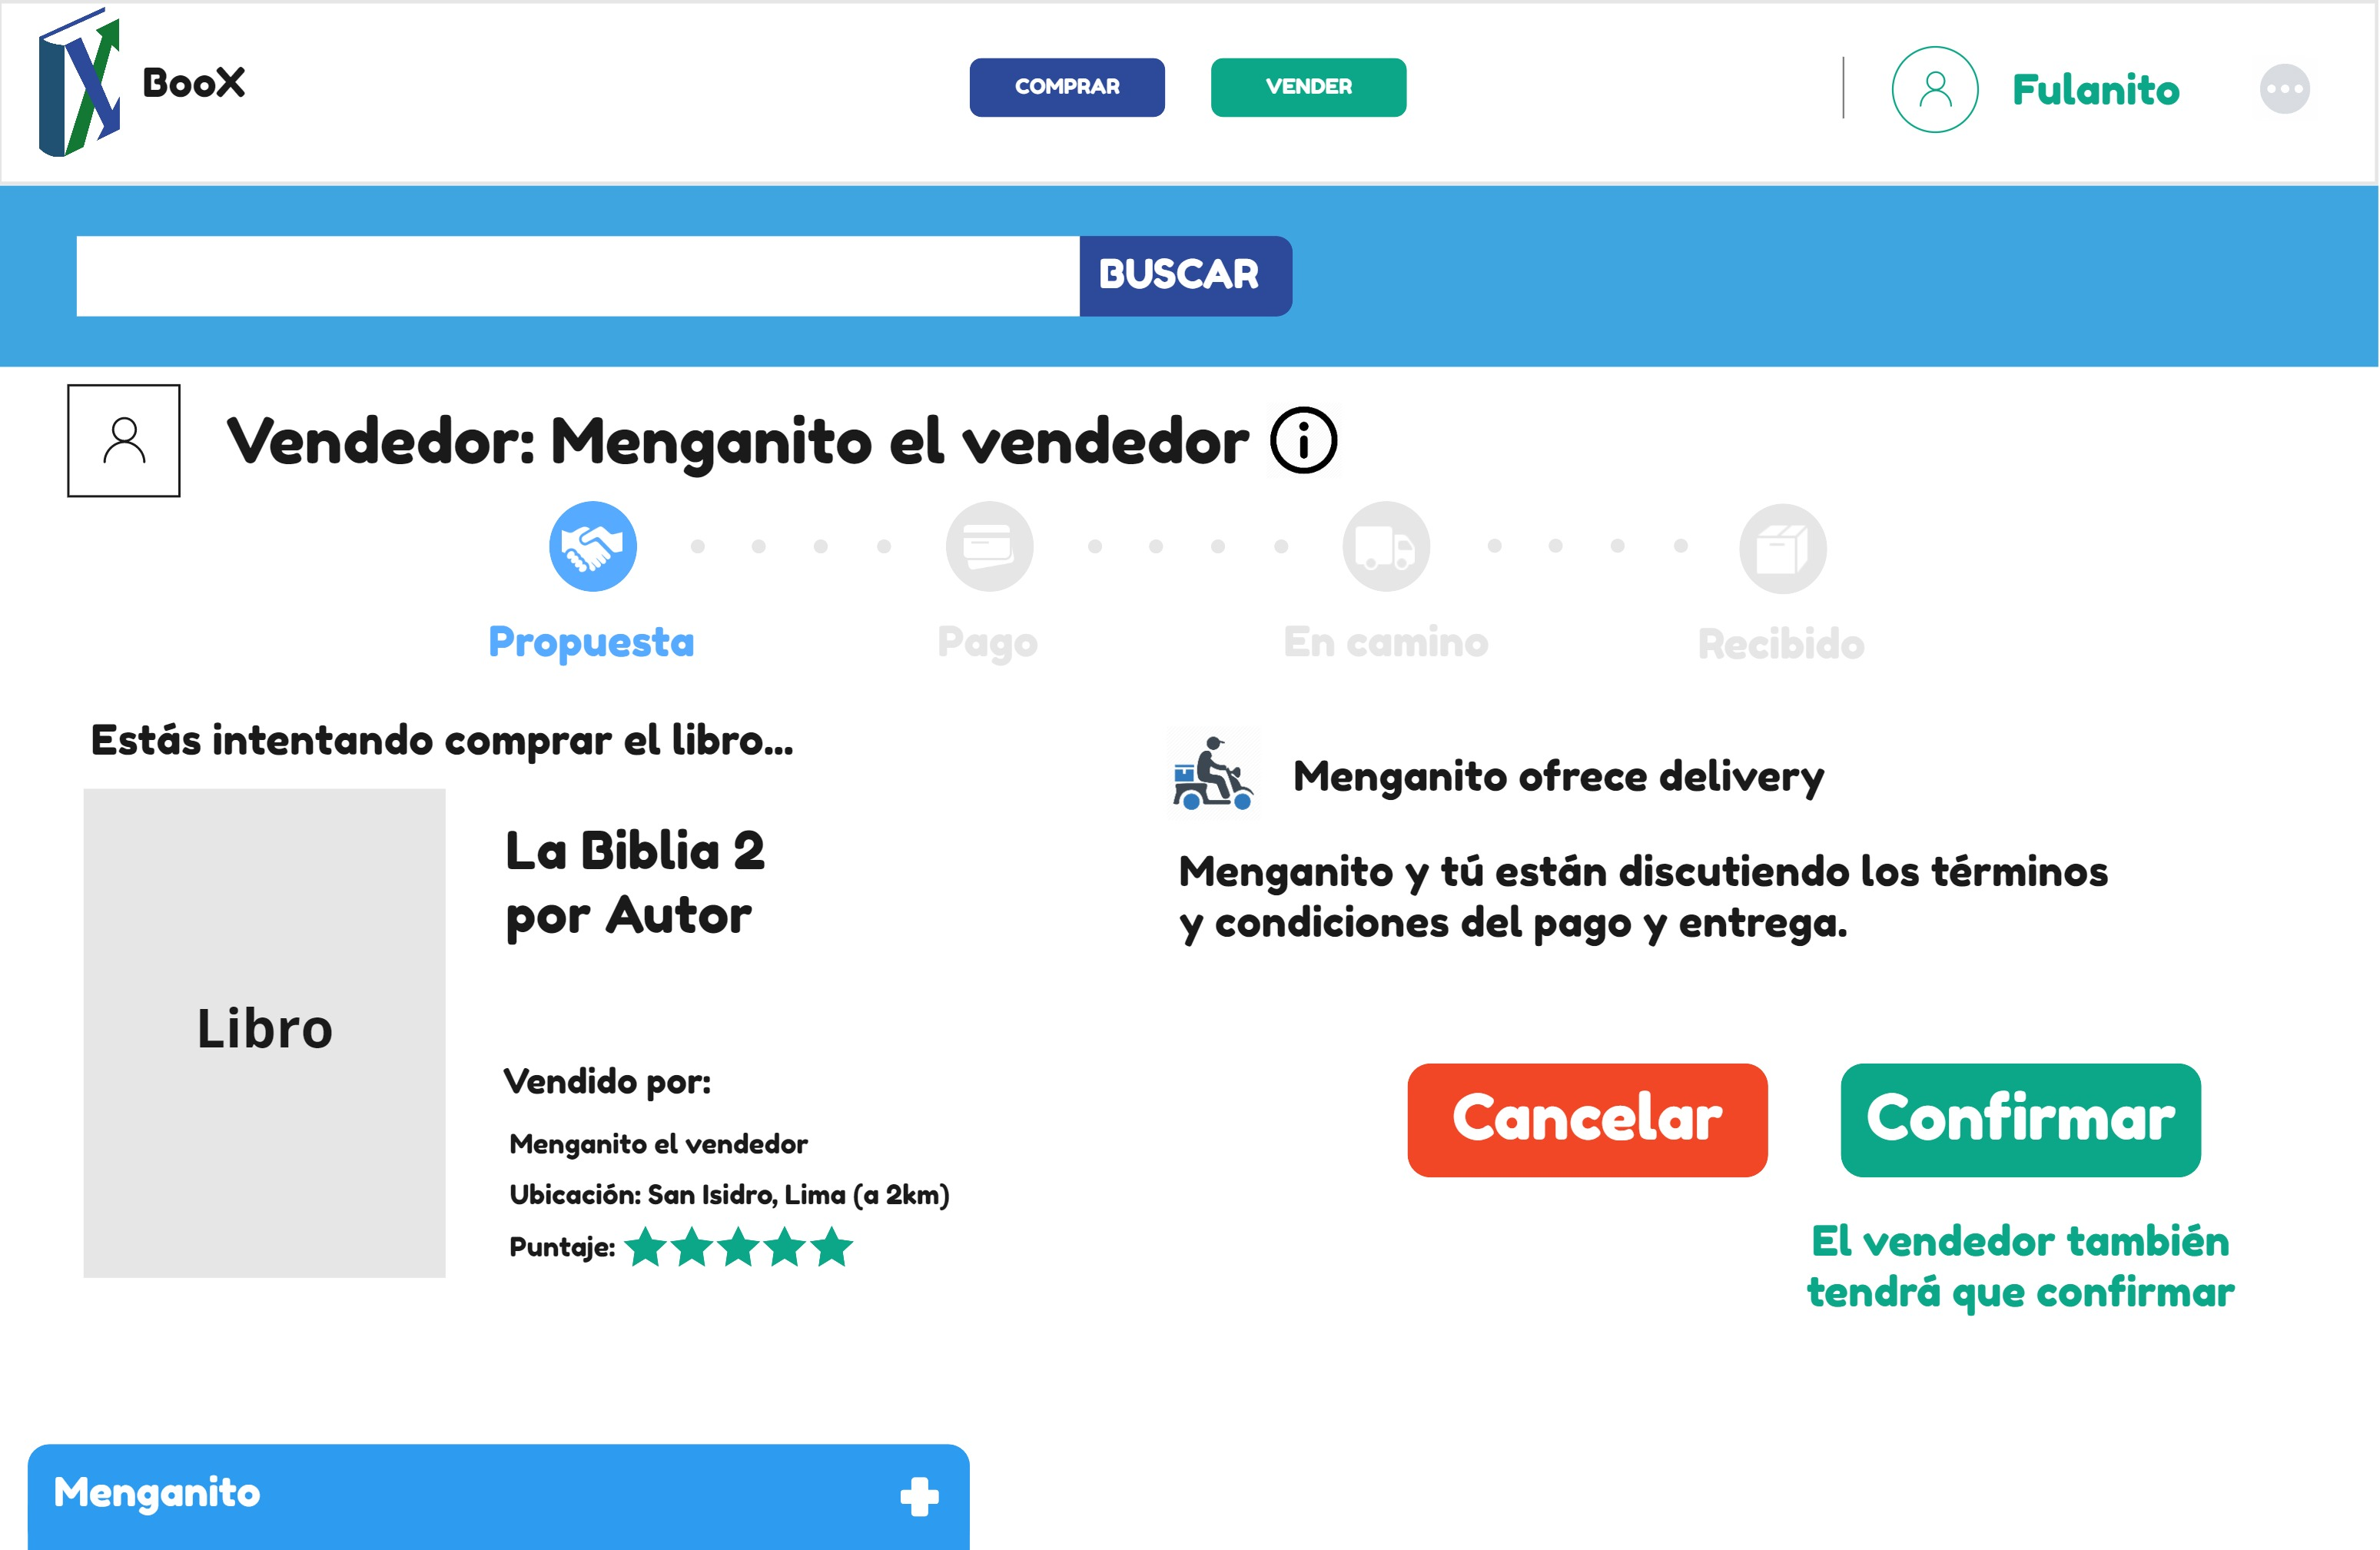
\includegraphics[width=300pt]{img/mockups/Huascar Retrieval Team - Contactar vendedor - Propuesta.jpg}
\end{center}

After clicking on "Contact", the user can contact the seller via a live chat and after agreeing to a proposal (delivery or meeting point) click on "Confirm".\\

\begin{center}
    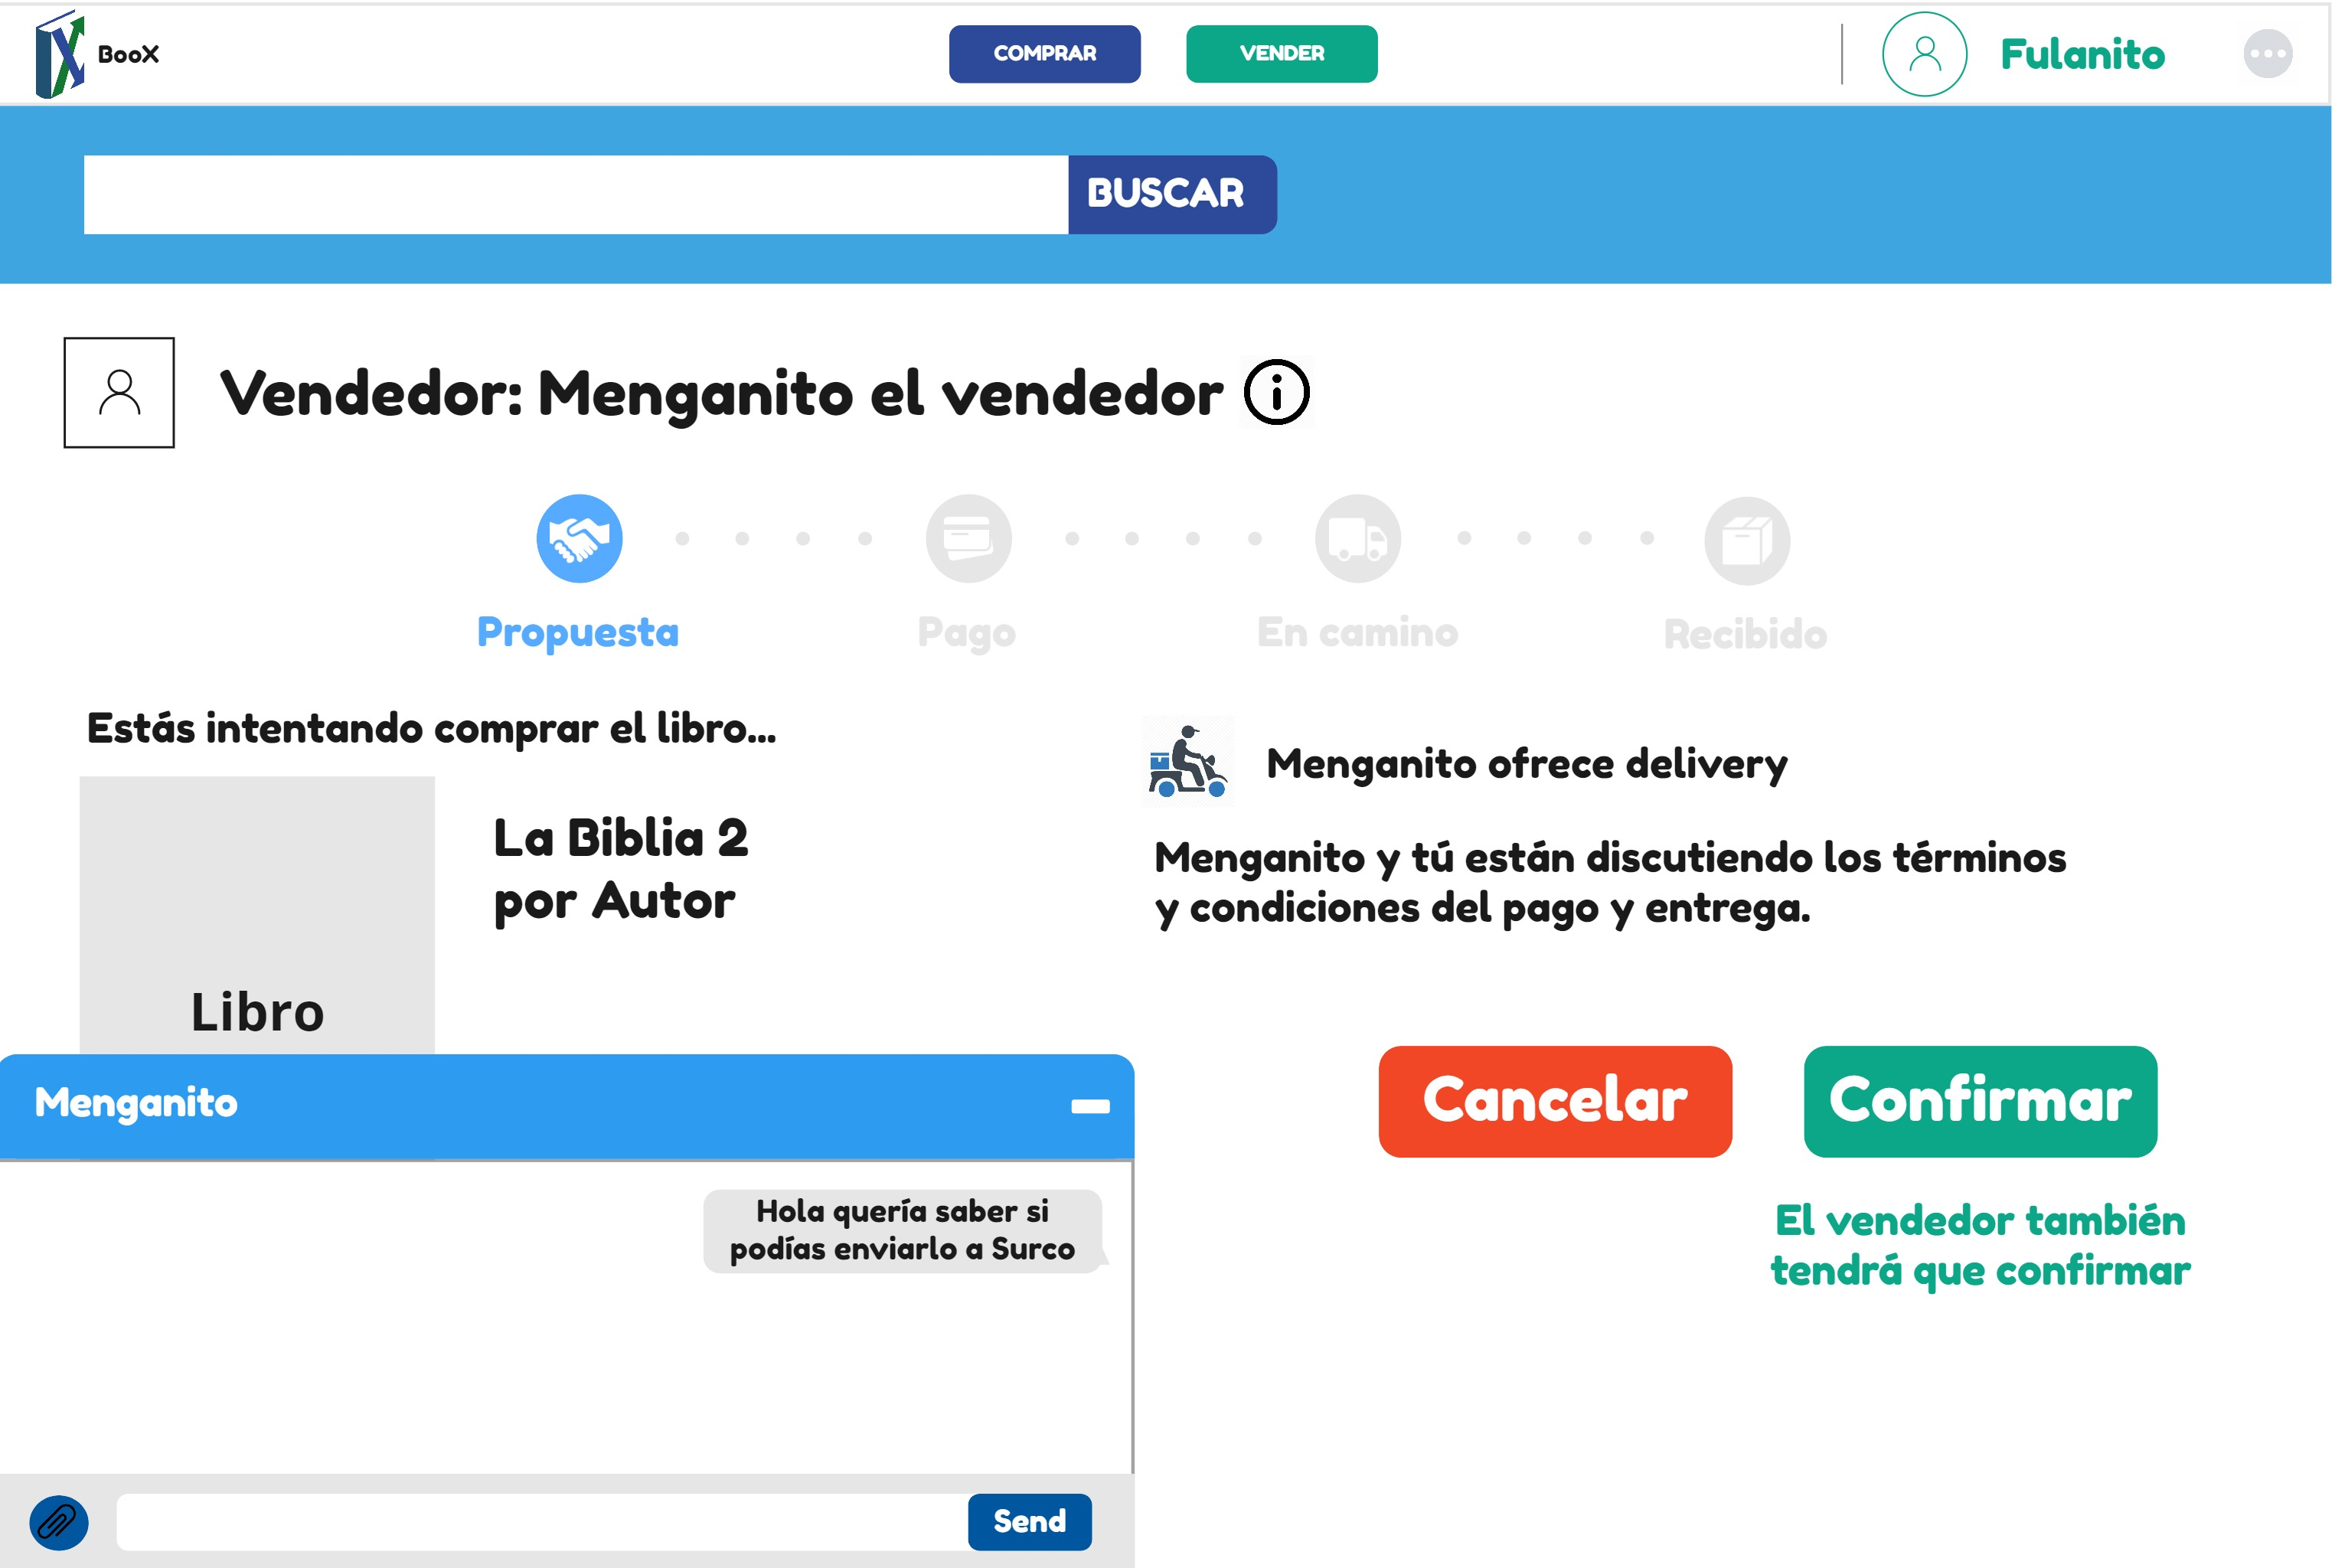
\includegraphics[width=300pt]{img/mockups/Huascar Retrieval Team - Copy of Contactar vendedor - Propuesta.jpg}
    \end{center}
    \subsubsection*{}
    \begin{center}
    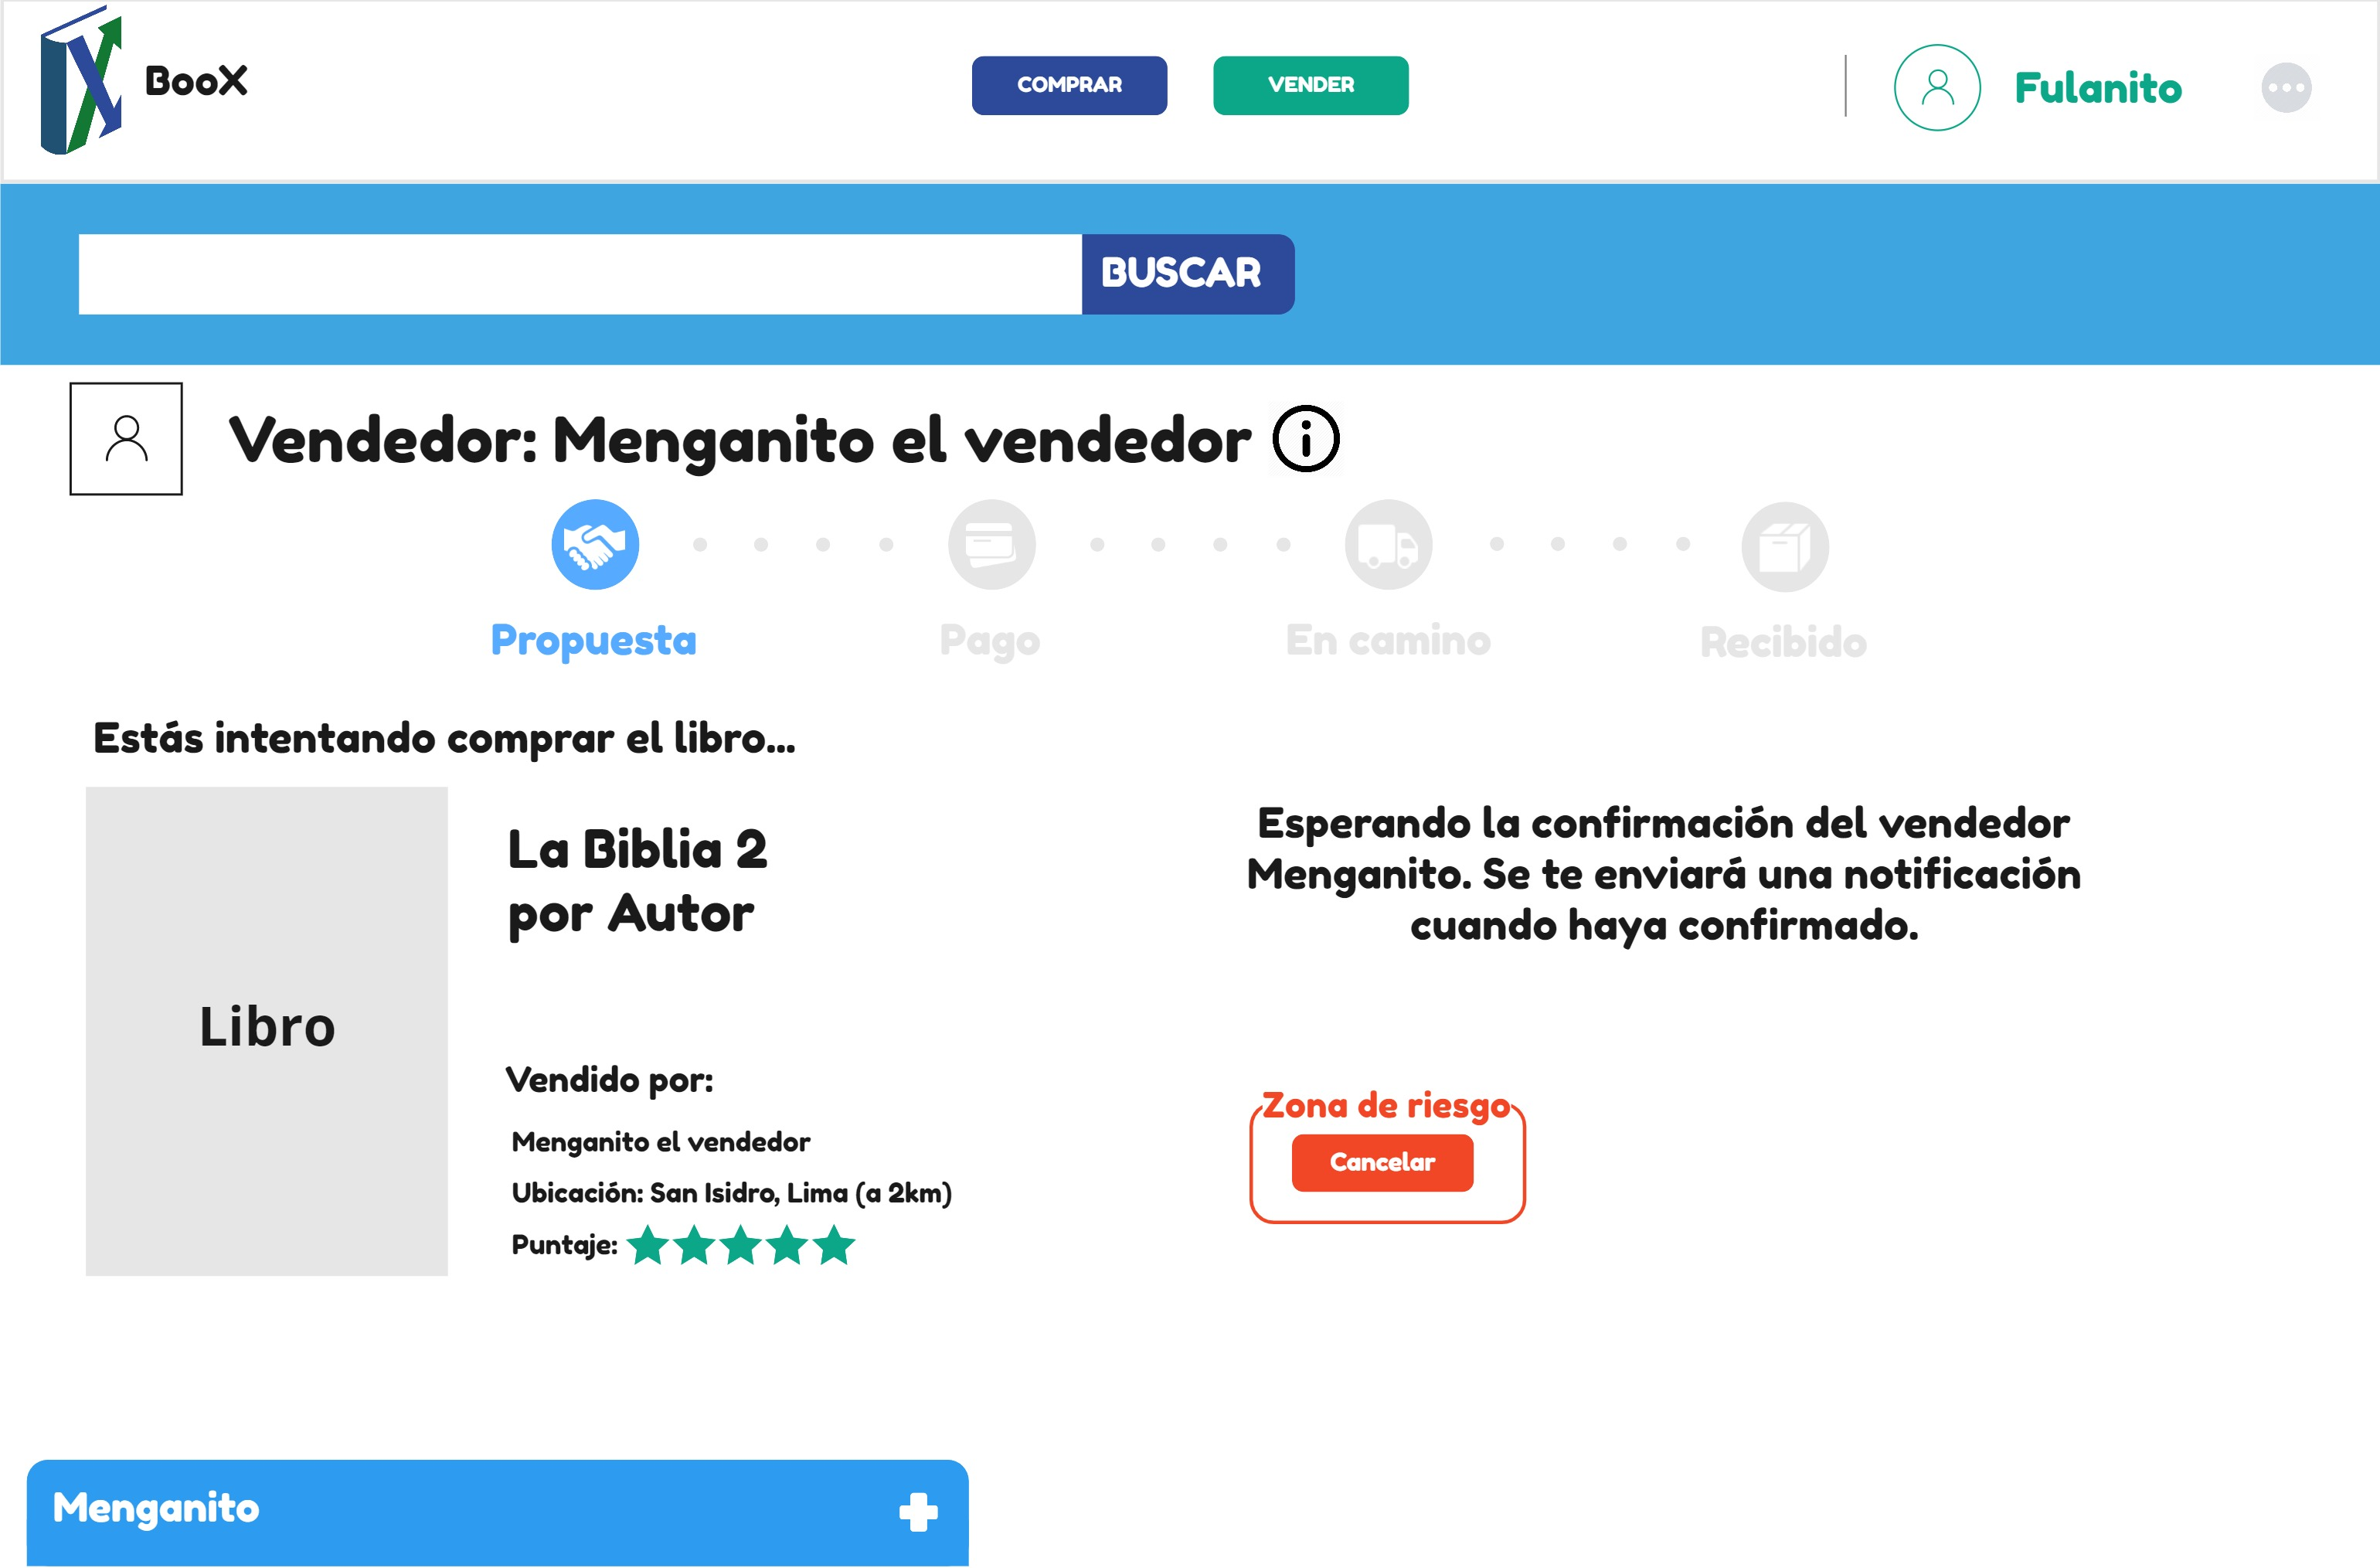
\includegraphics[width=300pt]{img/mockups/Huascar Retrieval Team - Copy of Contactar vendedor - Propuesta (1).jpg}
\end{center}


On the other side, the seller receives a notification when he or she is contacted\footnote{The notification is shown with a red dot on the user icon. A message appears on hover} and needs to confirm the proposal.\\

\begin{center}
    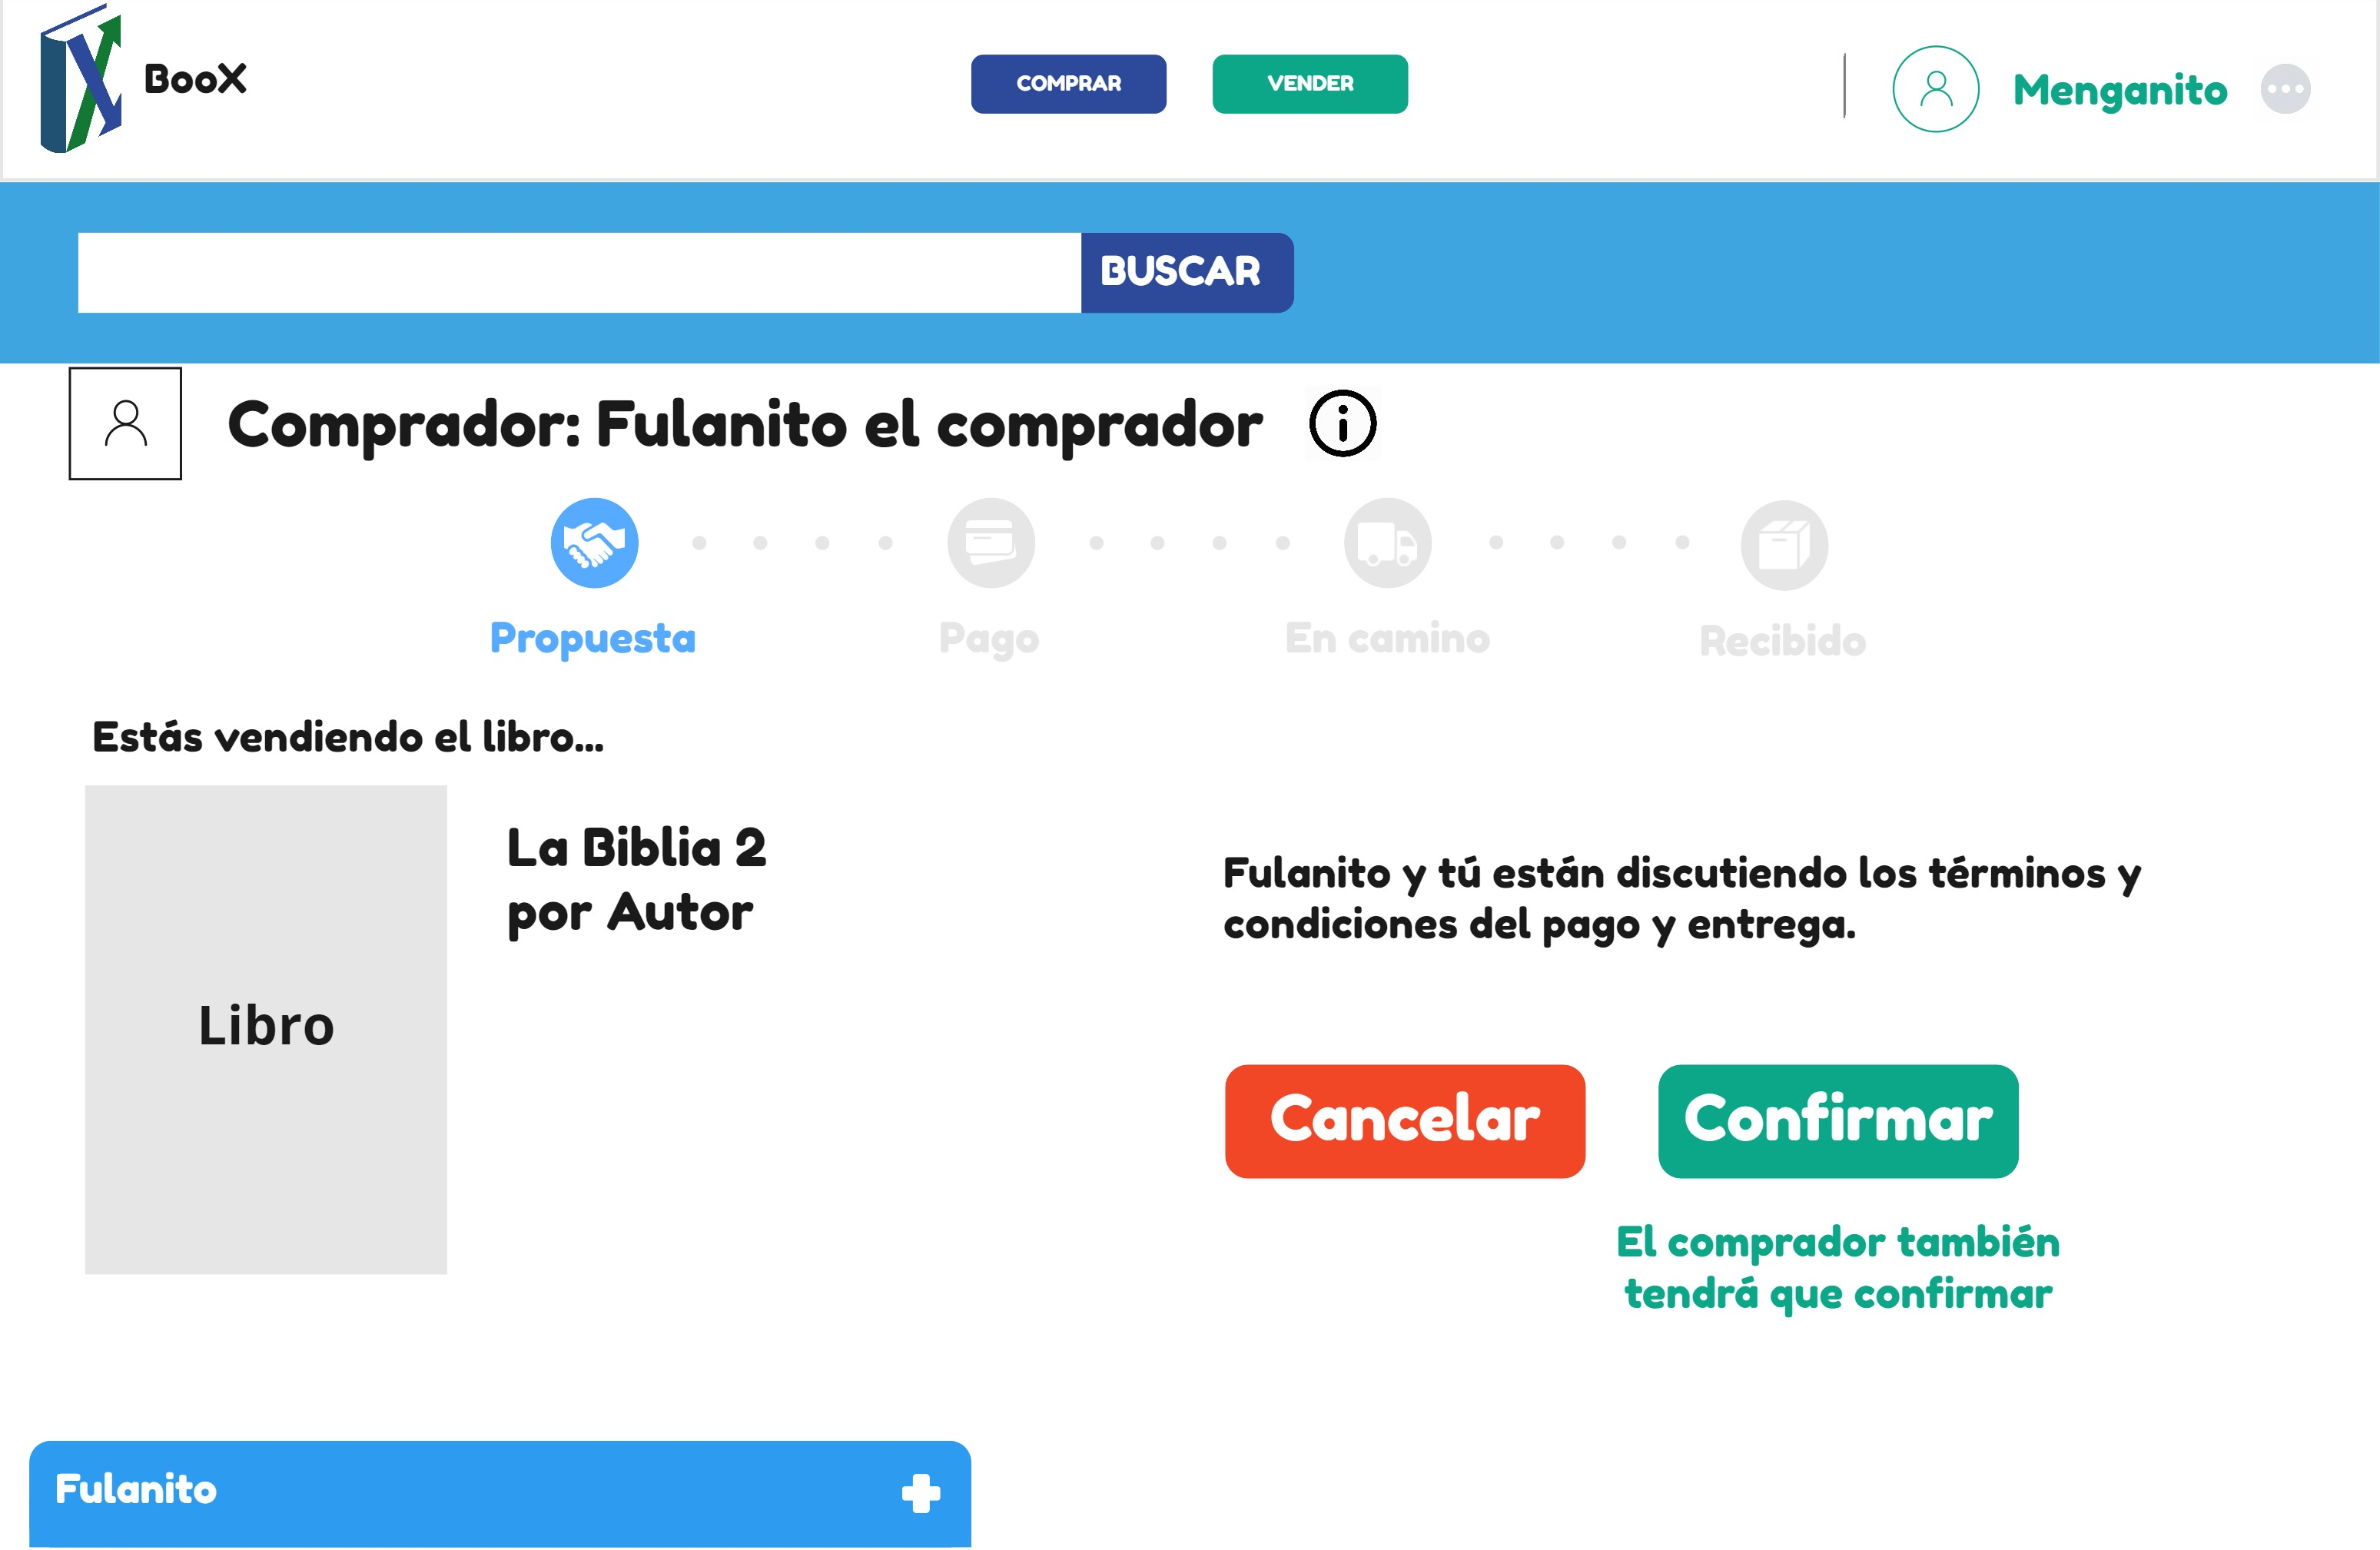
\includegraphics[width=300pt]{img/mockups/Huascar Retrieval Team - Vendedor siendo contactado (1).jpg}
\end{center}

Before being contacted, the seller had to add a book to sell. This is done by clicking on "Vender" button on the header or clicking on the upper right corner after logging in, which sends the user to his or her dashboard.

\begin{center}
    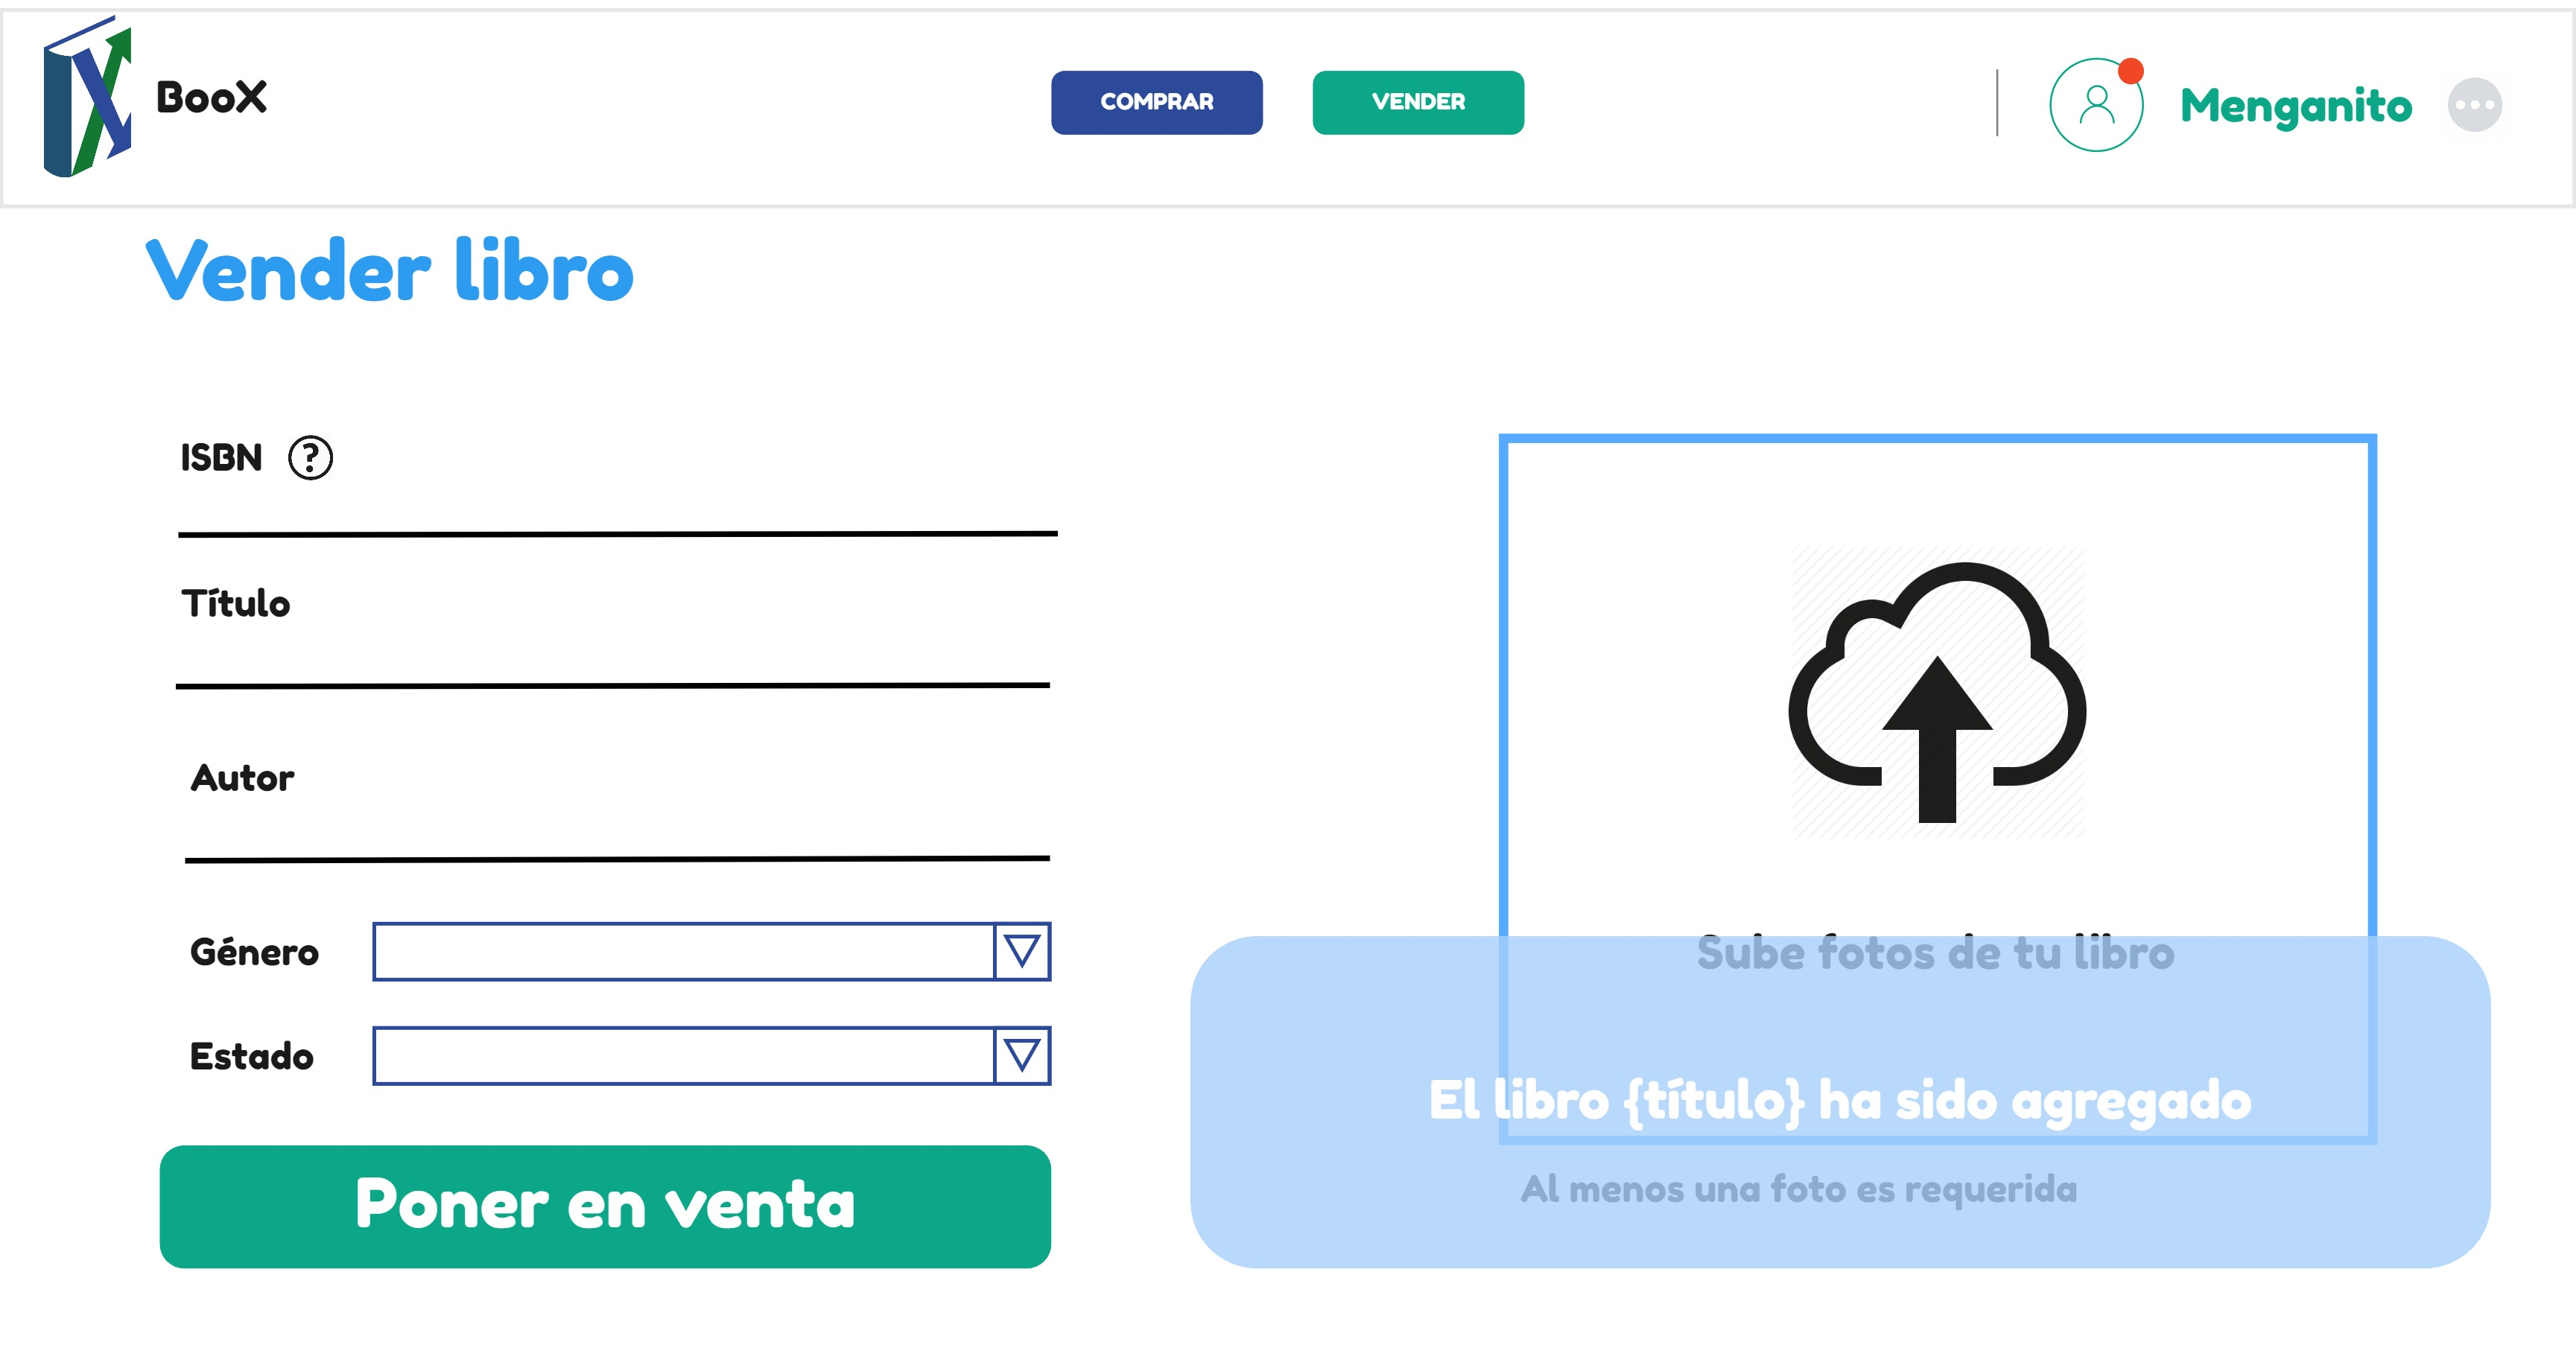
\includegraphics[width=300pt]{img/mockups/Huascar Retrieval Team - Copy of Dashboard.jpg}
\end{center}

Since every user can be a seller and a buyer, the dashboard contains this three options. If the user hasn't sold or bought a book, a message with a "No hay libros disponibles" is displayed instead of an empty space.


\begin{center}
    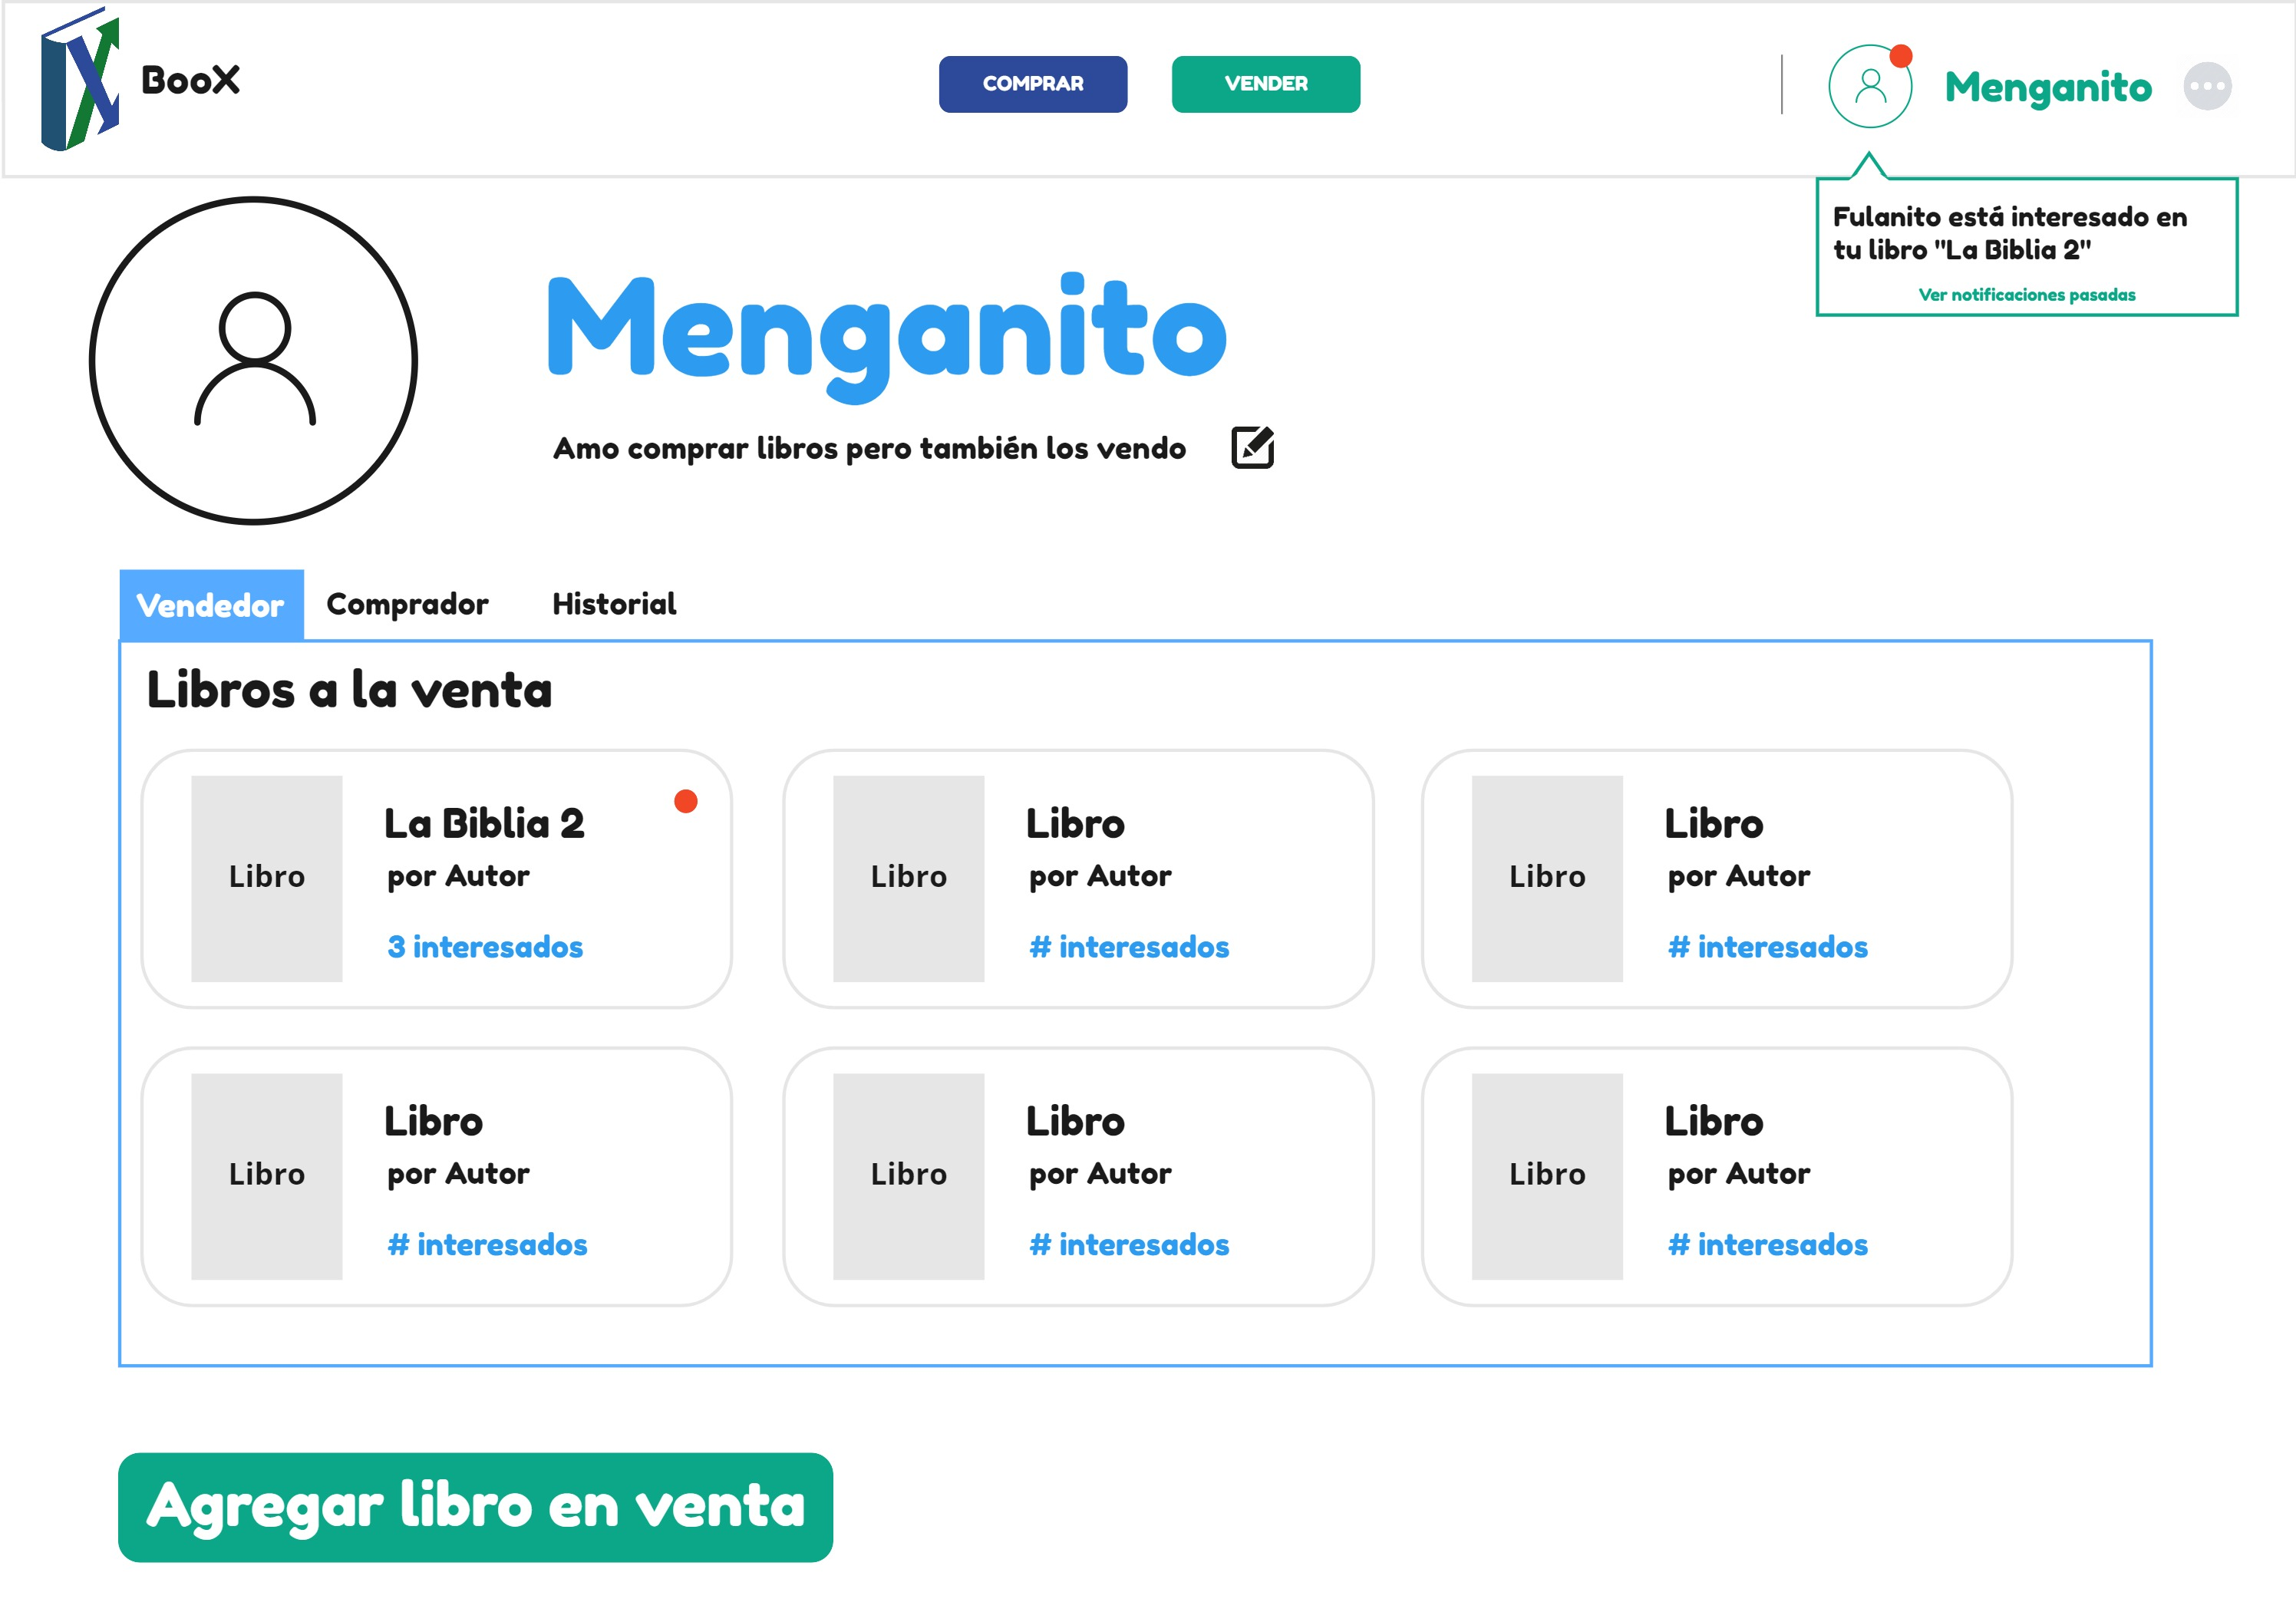
\includegraphics[width=300pt]{img/mockups/Huascar Retrieval Team - Dashboard vendedor.jpg}
    \end{center}
    \subsubsection*{}
    \begin{center}
    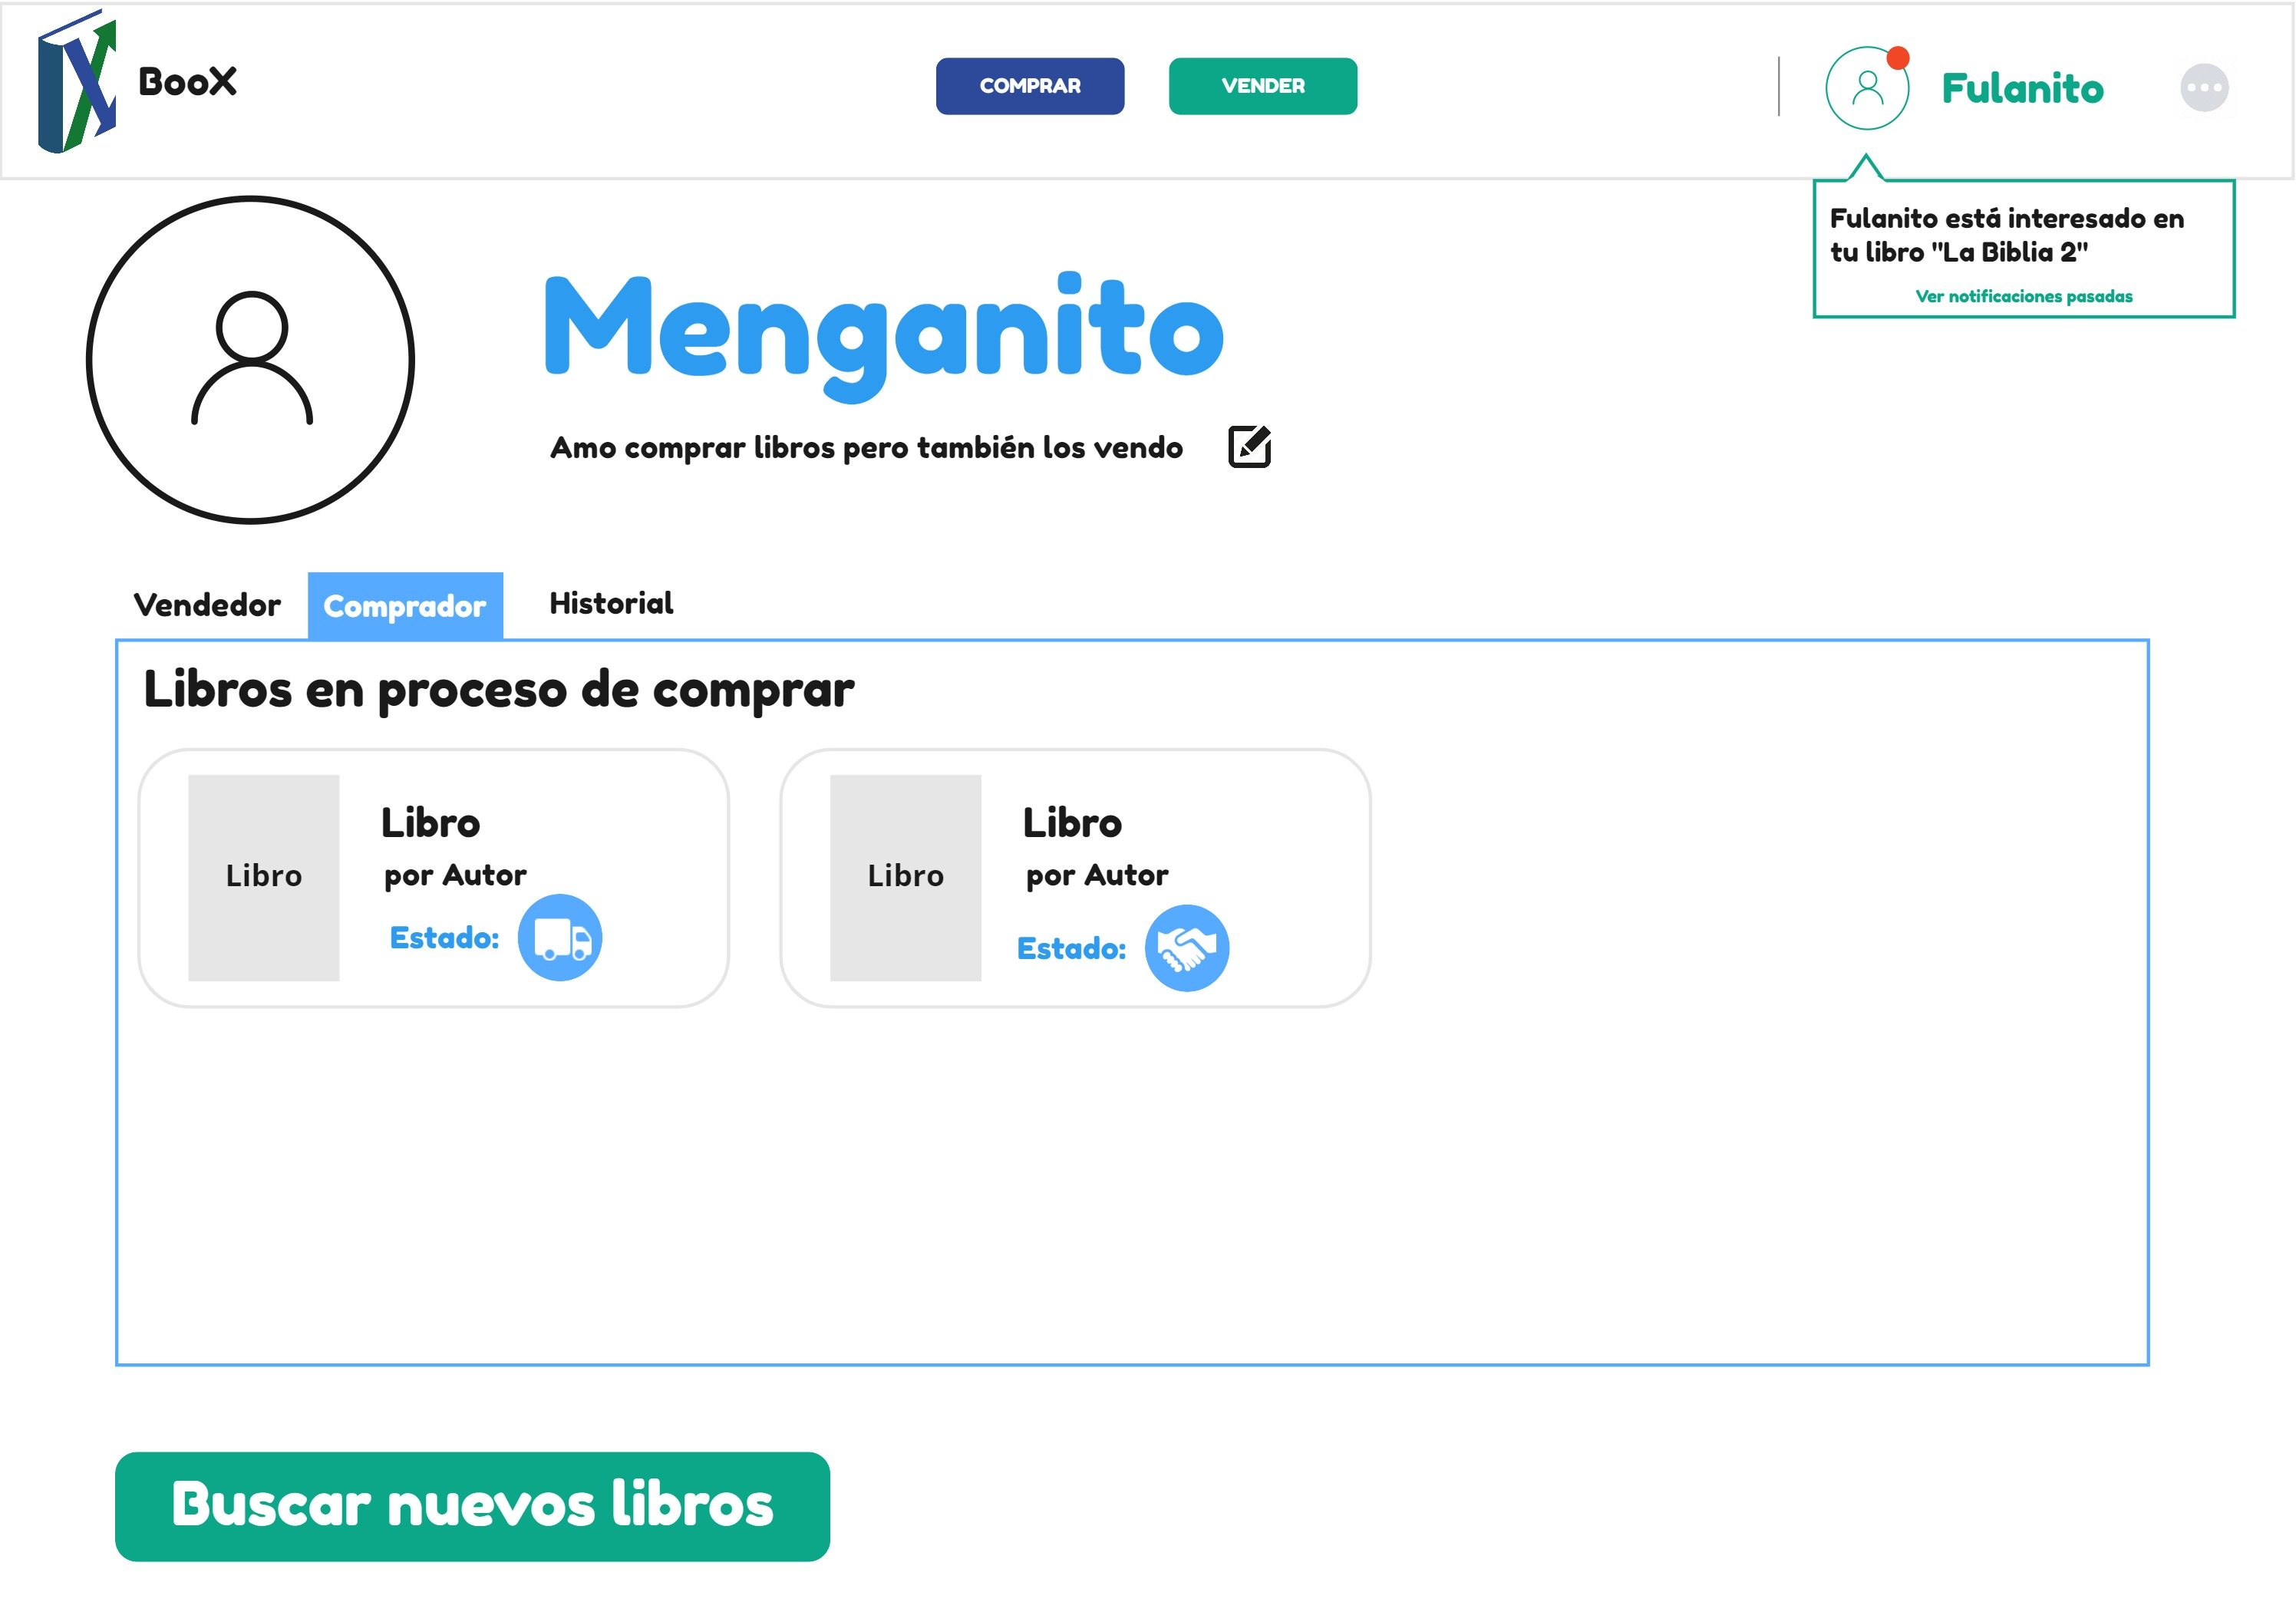
\includegraphics[width=300pt]{img/mockups/Huascar Retrieval Team - Dashboard comprador.jpg}
    \end{center}
    \subsubsection*{}
    \begin{center}
    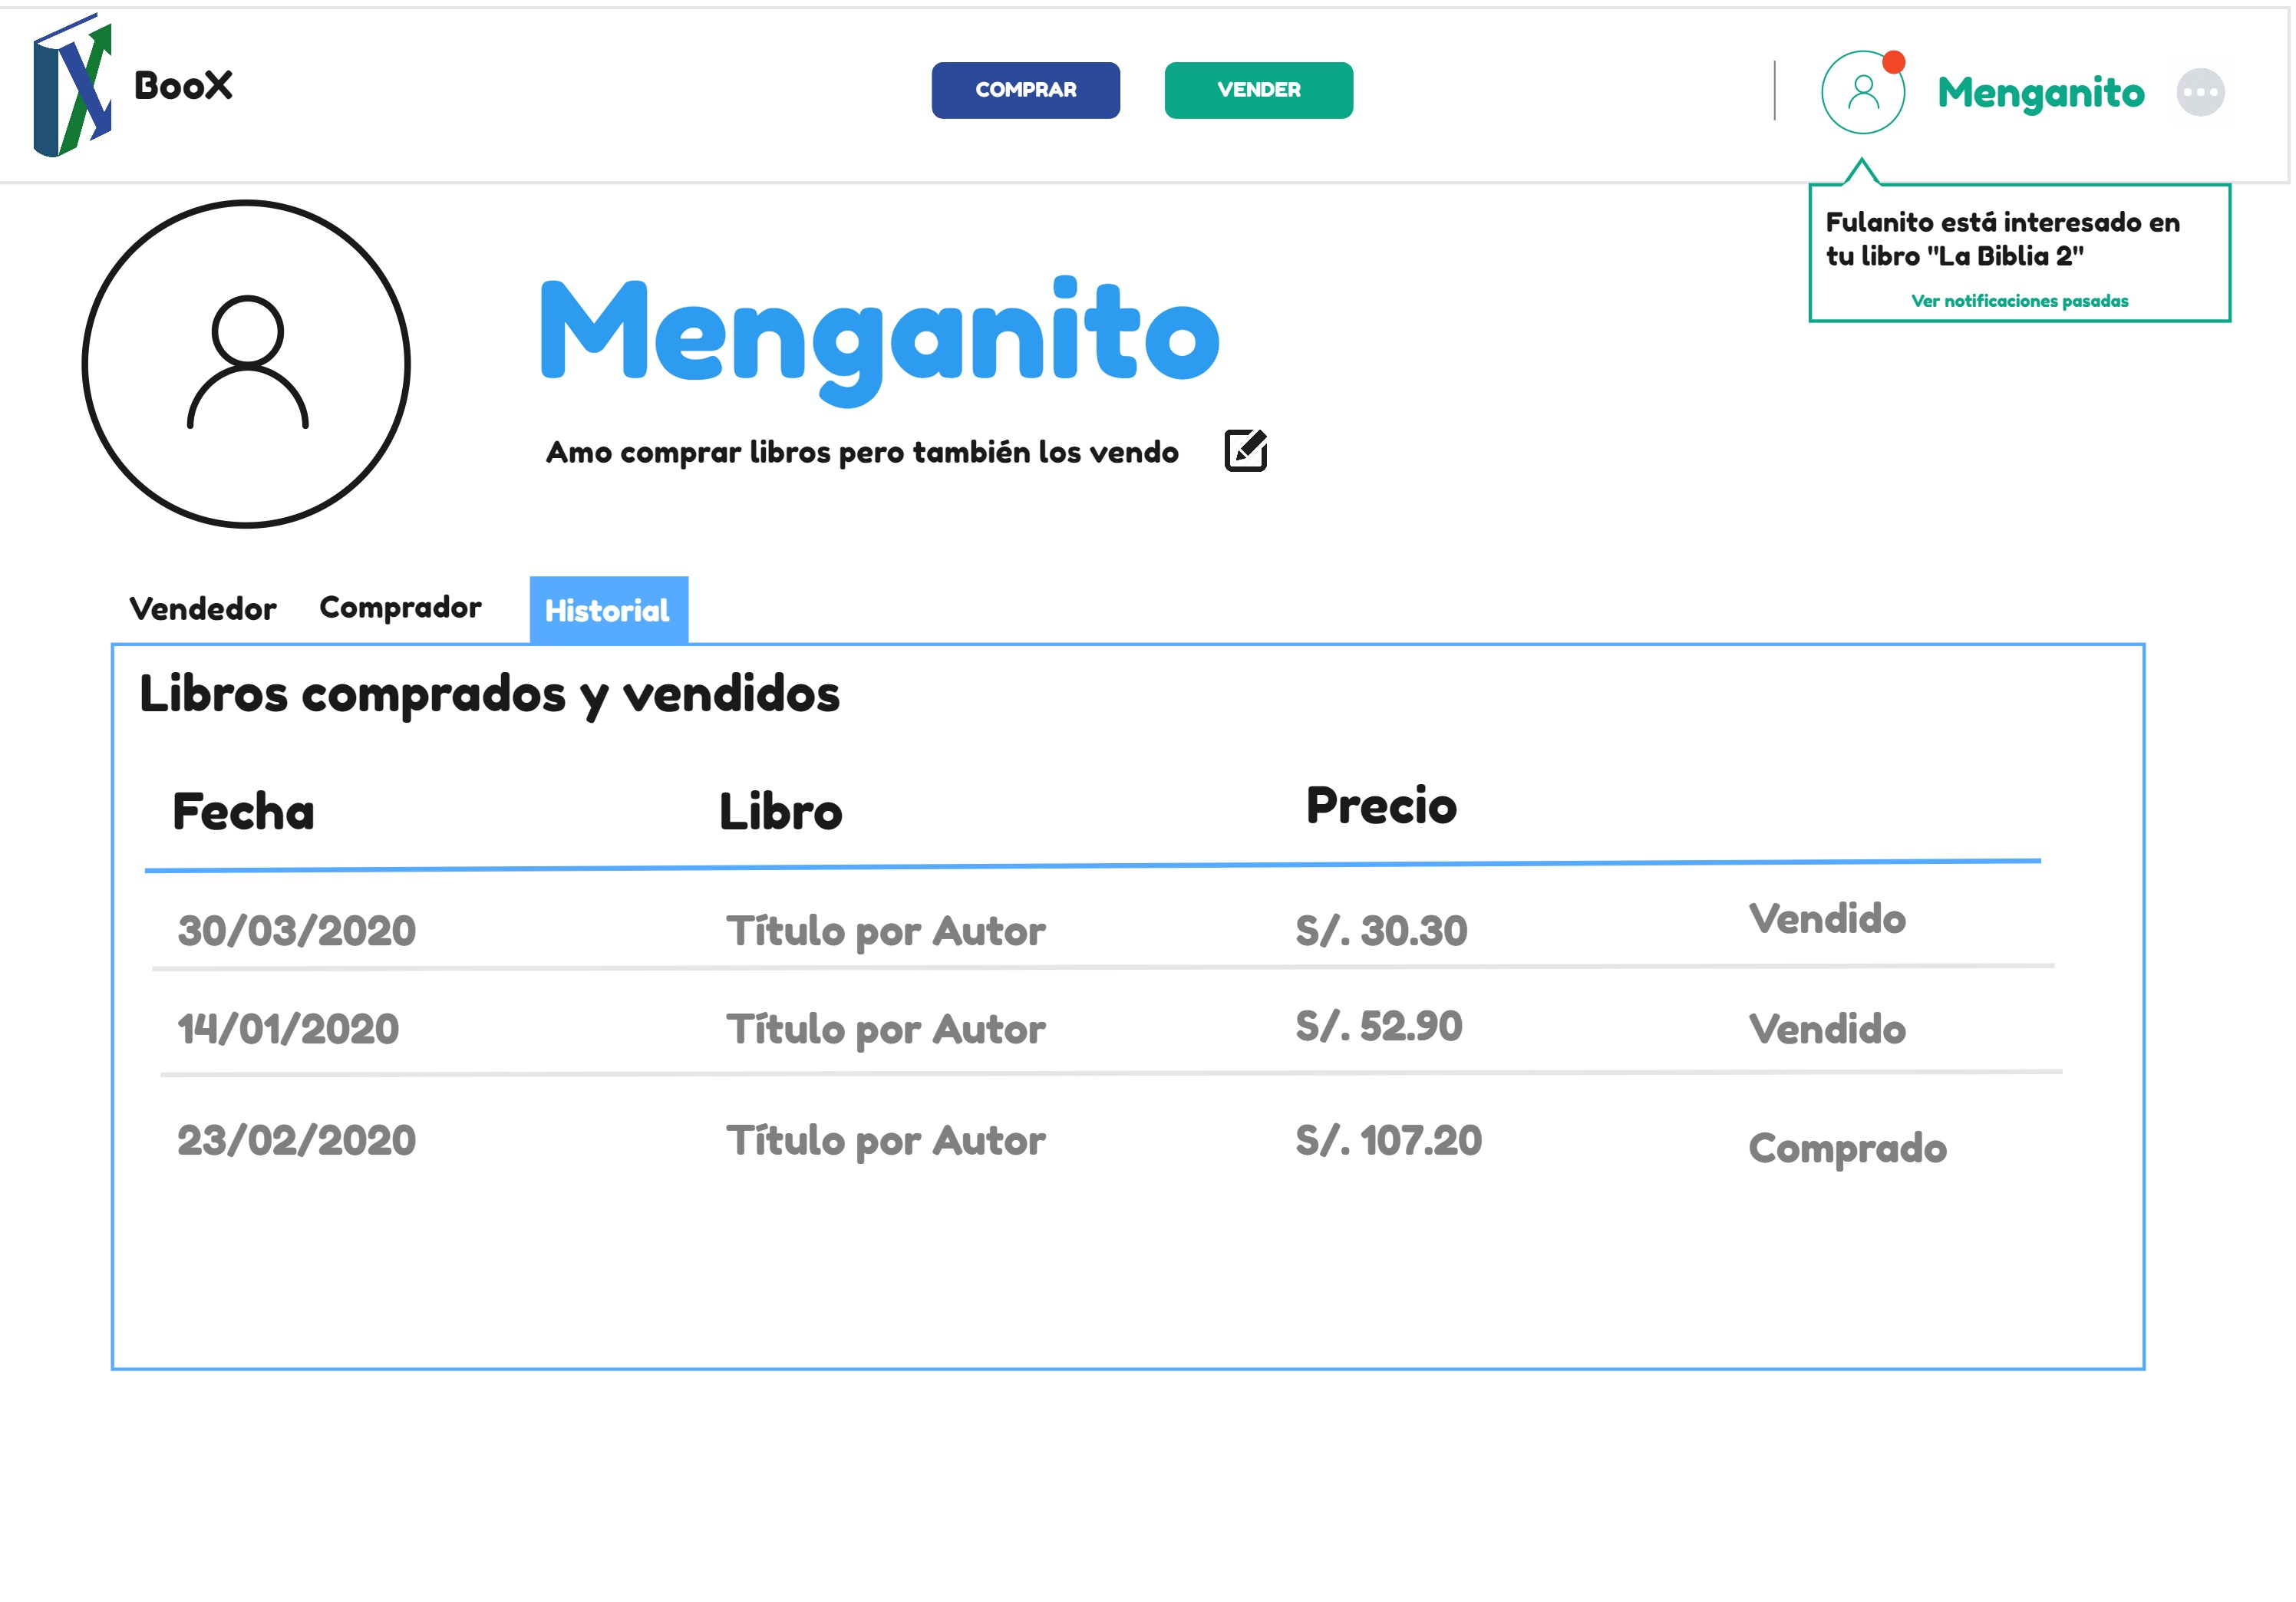
\includegraphics[width=300pt]{img/mockups/Huascar Retrieval Team - Dashboard historial.jpg}
\end{center}

If a book is clicked on the seller tab on the dashboard, a page like the following is displayed. If a book is pressed in the buyers tab, the pages presented below appear depending on the stage of the purchase.

\begin{center}
    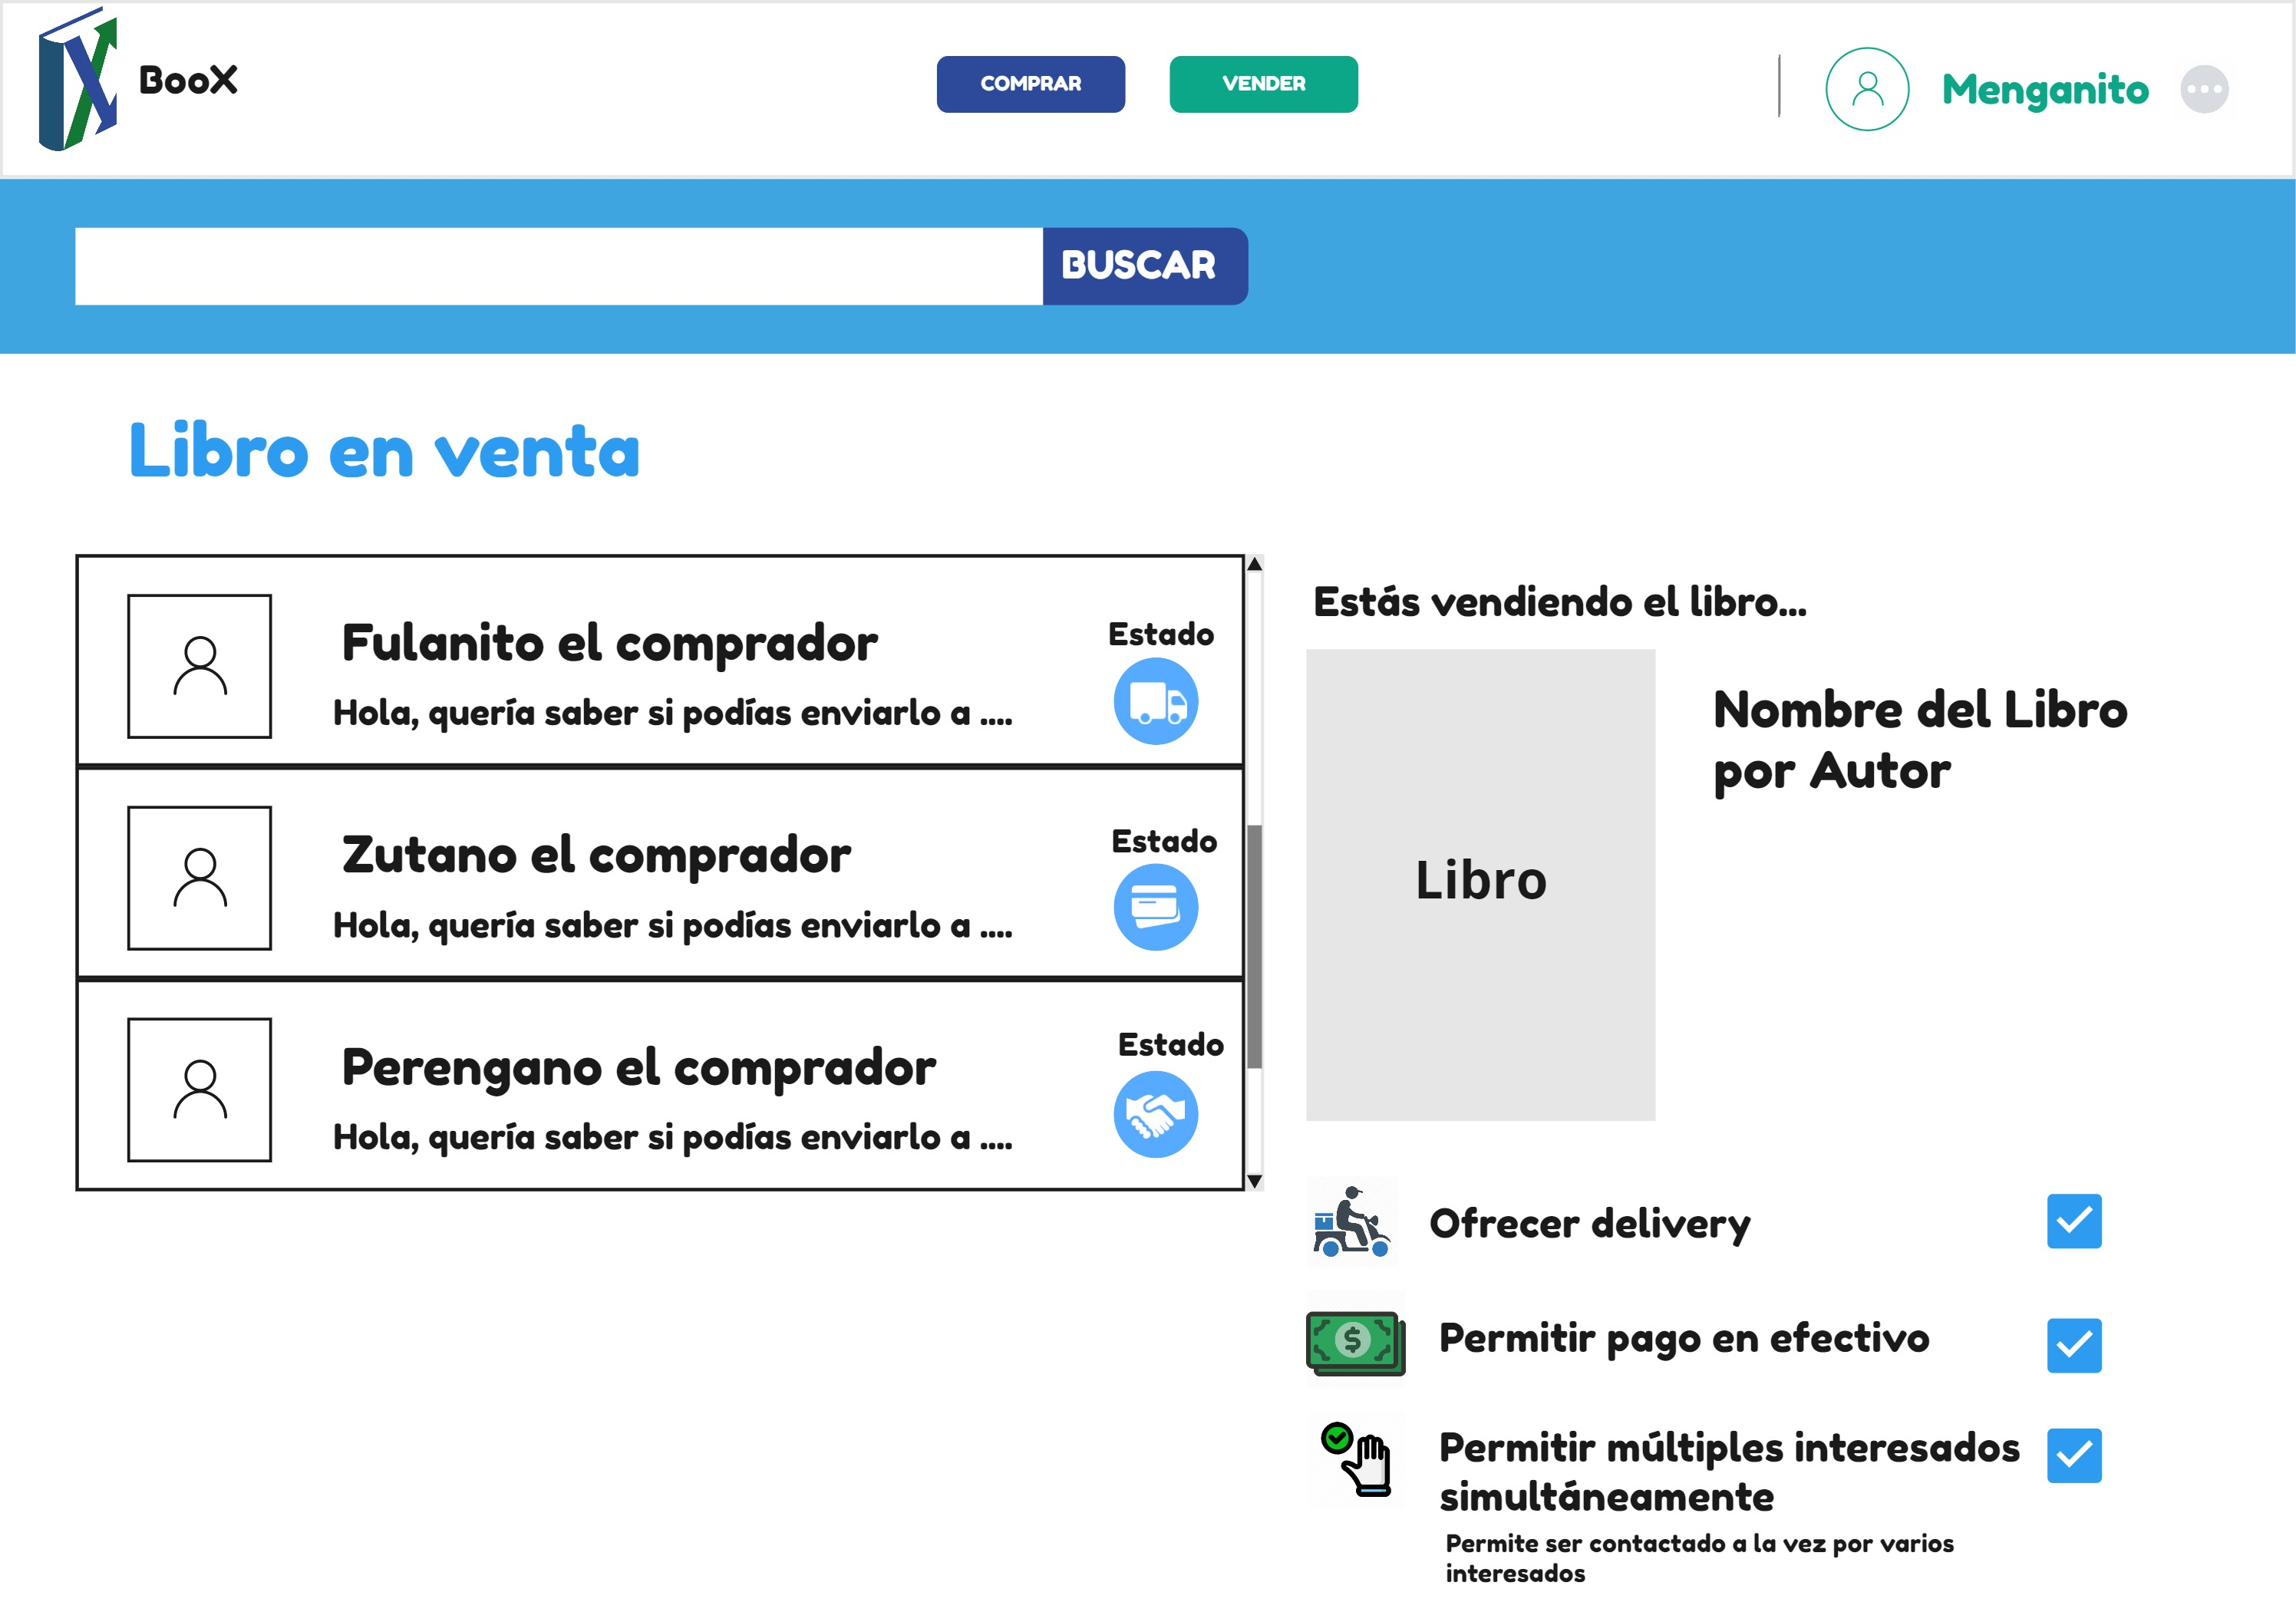
\includegraphics[width=300pt]{img/mockups/Huascar Retrieval Team - Vendedor siendo contactado.jpg}
\end{center}

The next pages show the process to buy a book from the buyer's (Fulanito on the upper right corner) and seller's (Menganito on the upper right corner) perspective.

On the third stage, "En camino", the buyer is first presented with a first line of "Tu libro está en camino" and the seller with input boxes for a delivery address (in case it is being send by delivery and not meeting point) and additional information if needed (ex: tracking code of the package). Only after the seller confirms the delivery, the buyer gets the address where the package is or will be send and the additional information entered by the seller. The option of "change address" is also presented to the buyer, which sends a notification to the seller and can change the address if possible.

\begin{center}
    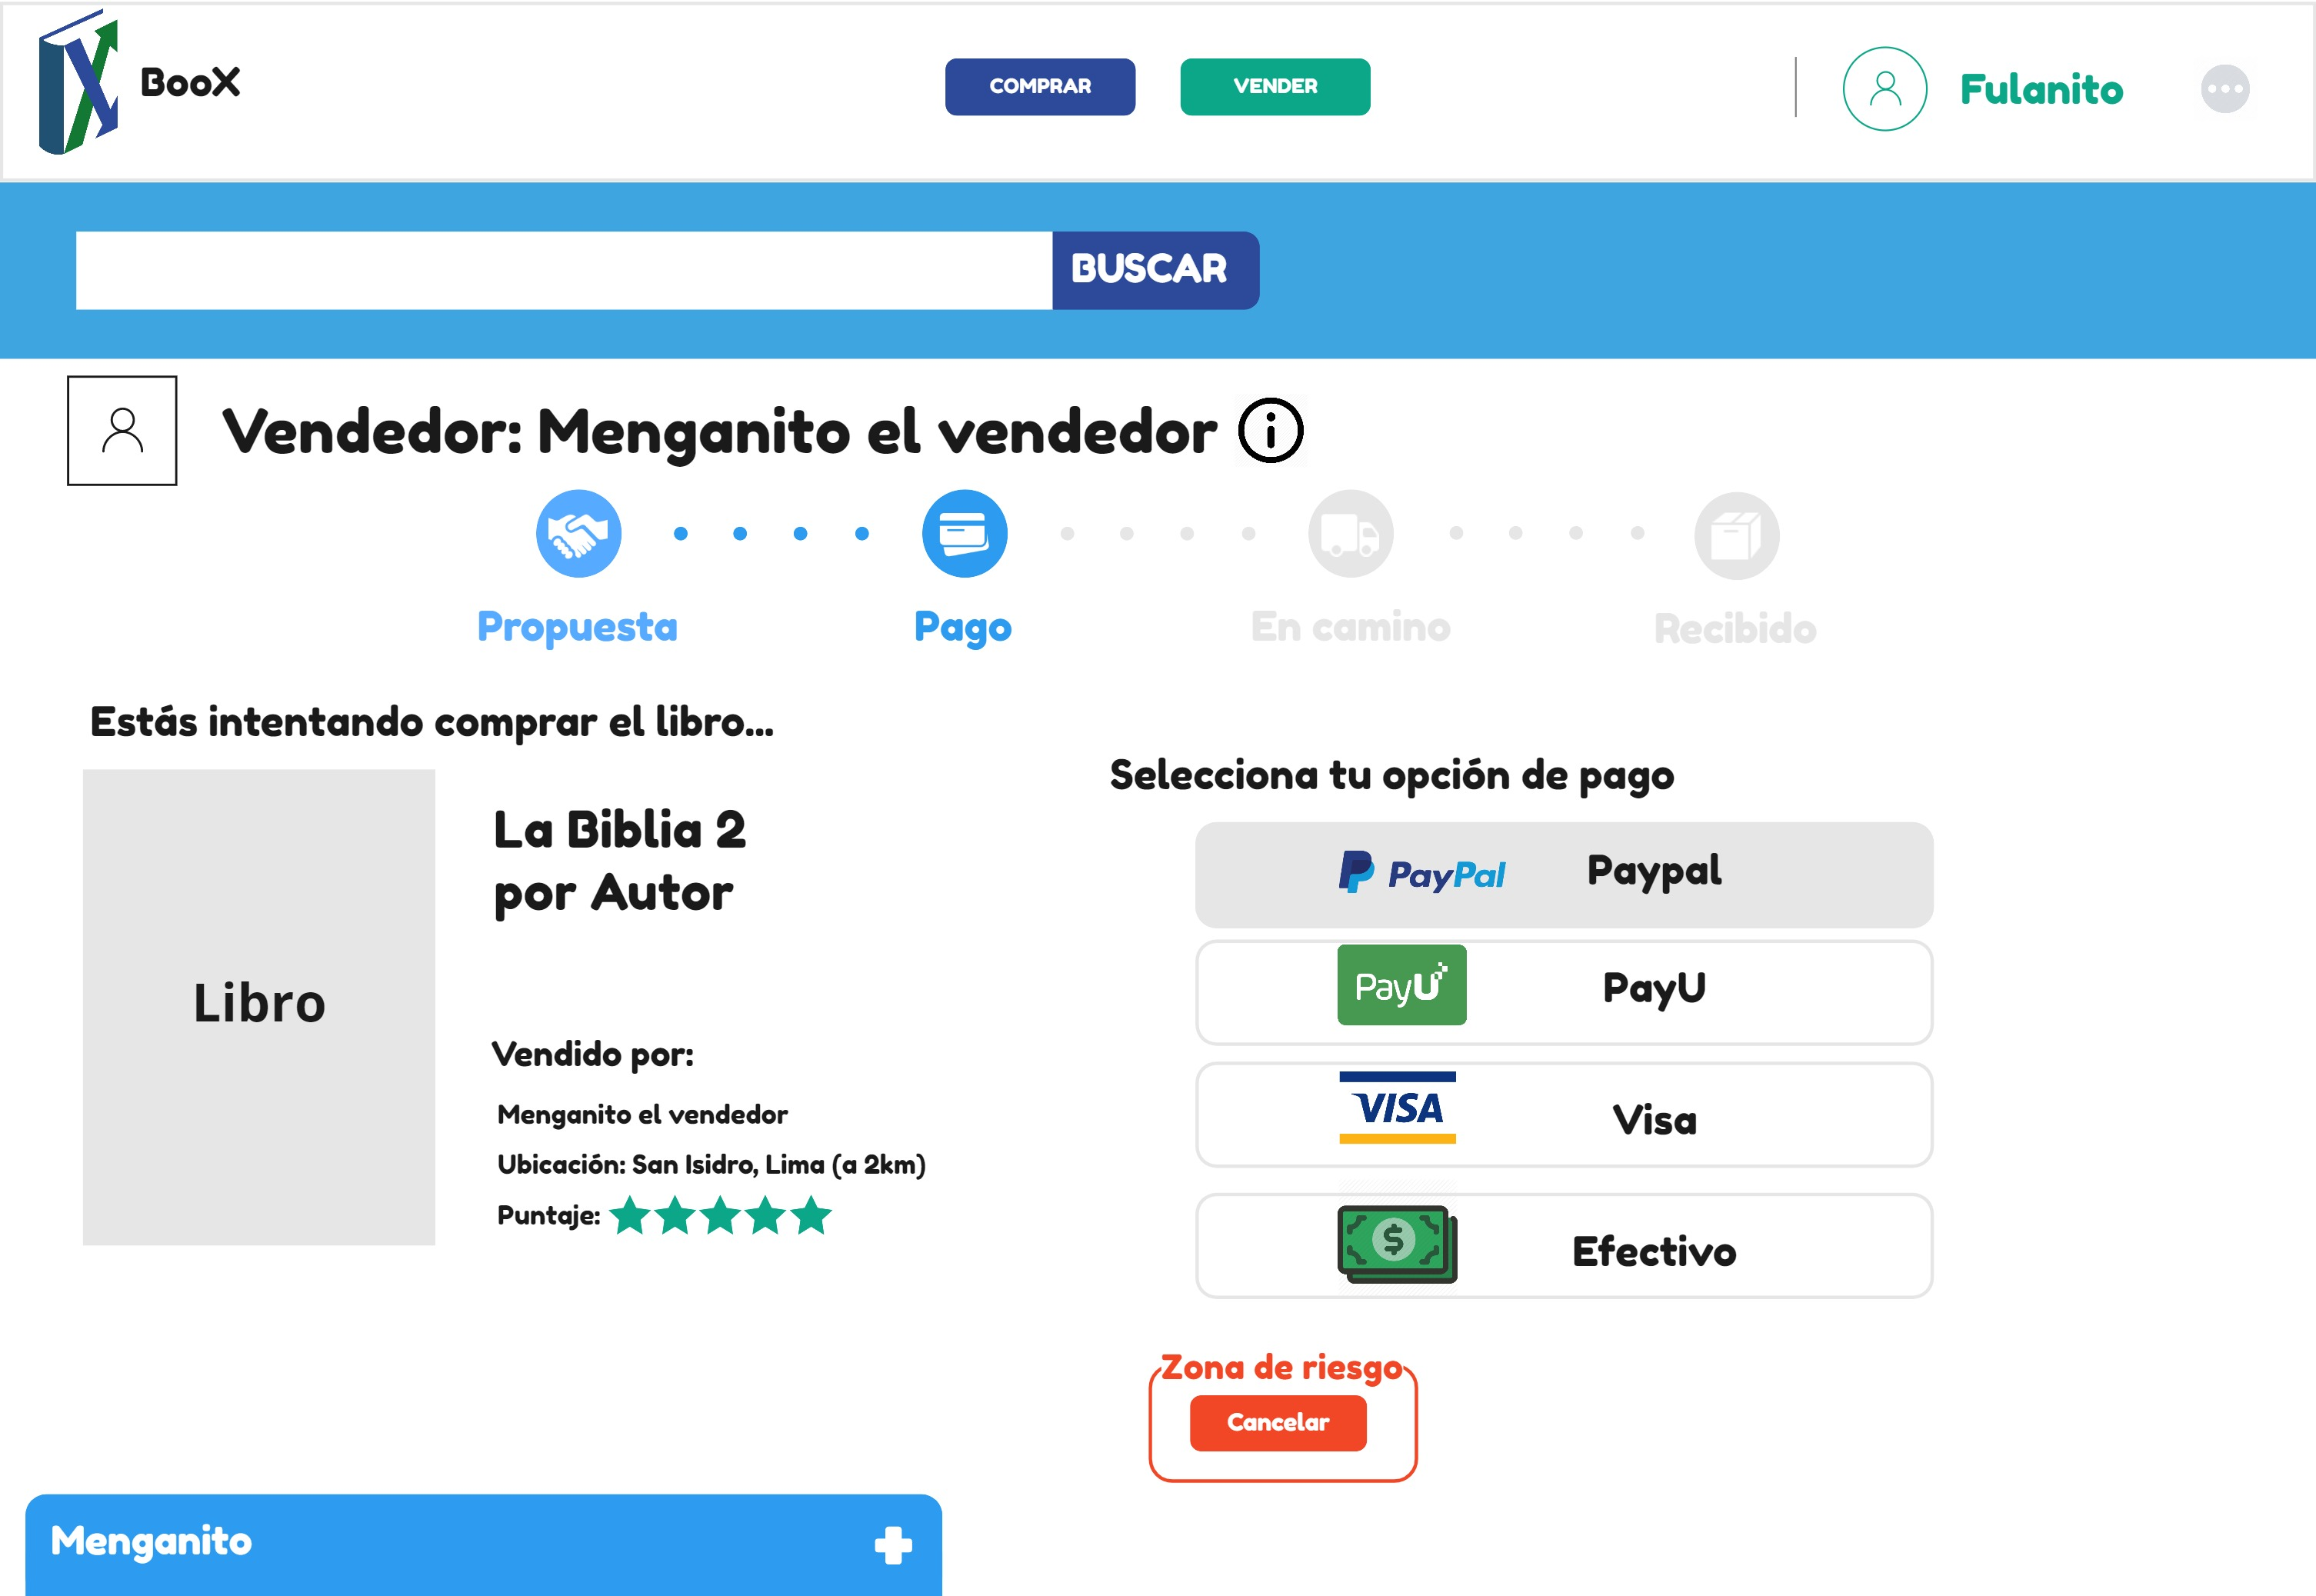
\includegraphics[width=300pt]{img/mockups/Huascar Retrieval Team - Contactar vendedor - Pago.jpg}
    \end{center}
    \subsubsection*{}
    \begin{center}
    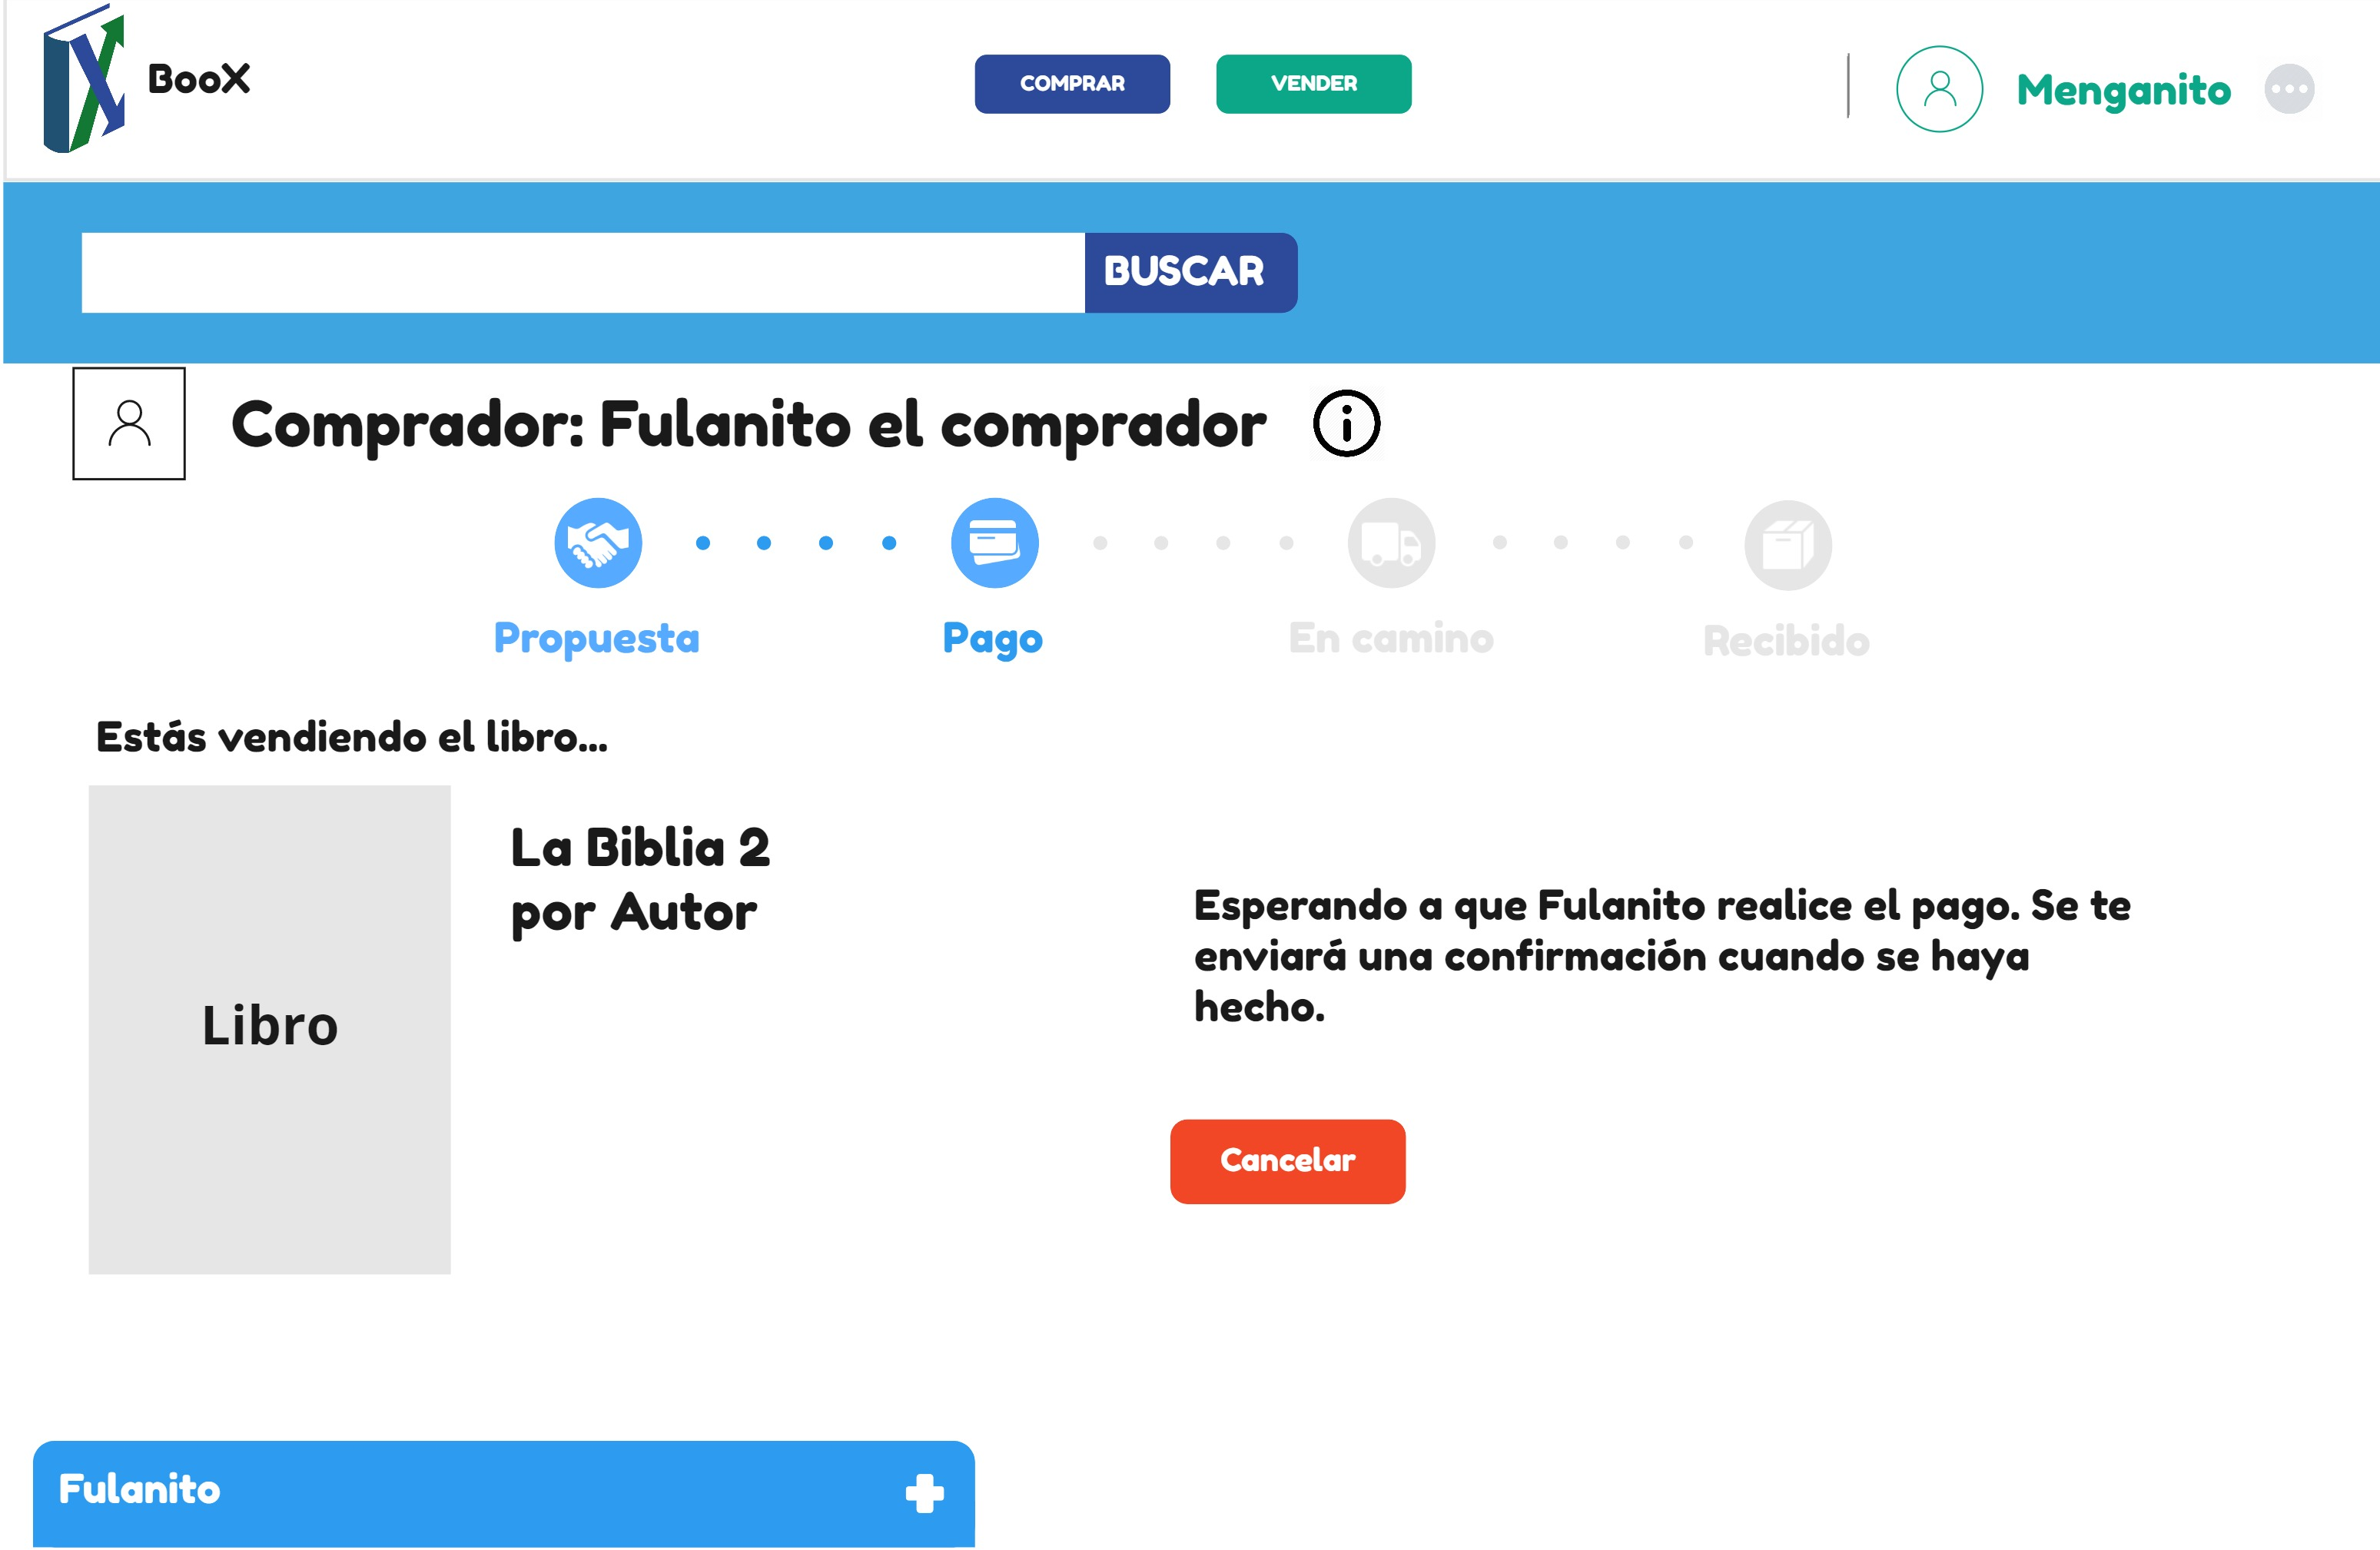
\includegraphics[width=300pt]{img/mockups/Huascar Retrieval Team - Vendedor siendo contactado (3).jpg}
    \end{center}
    \subsubsection*{}
    \begin{center}
    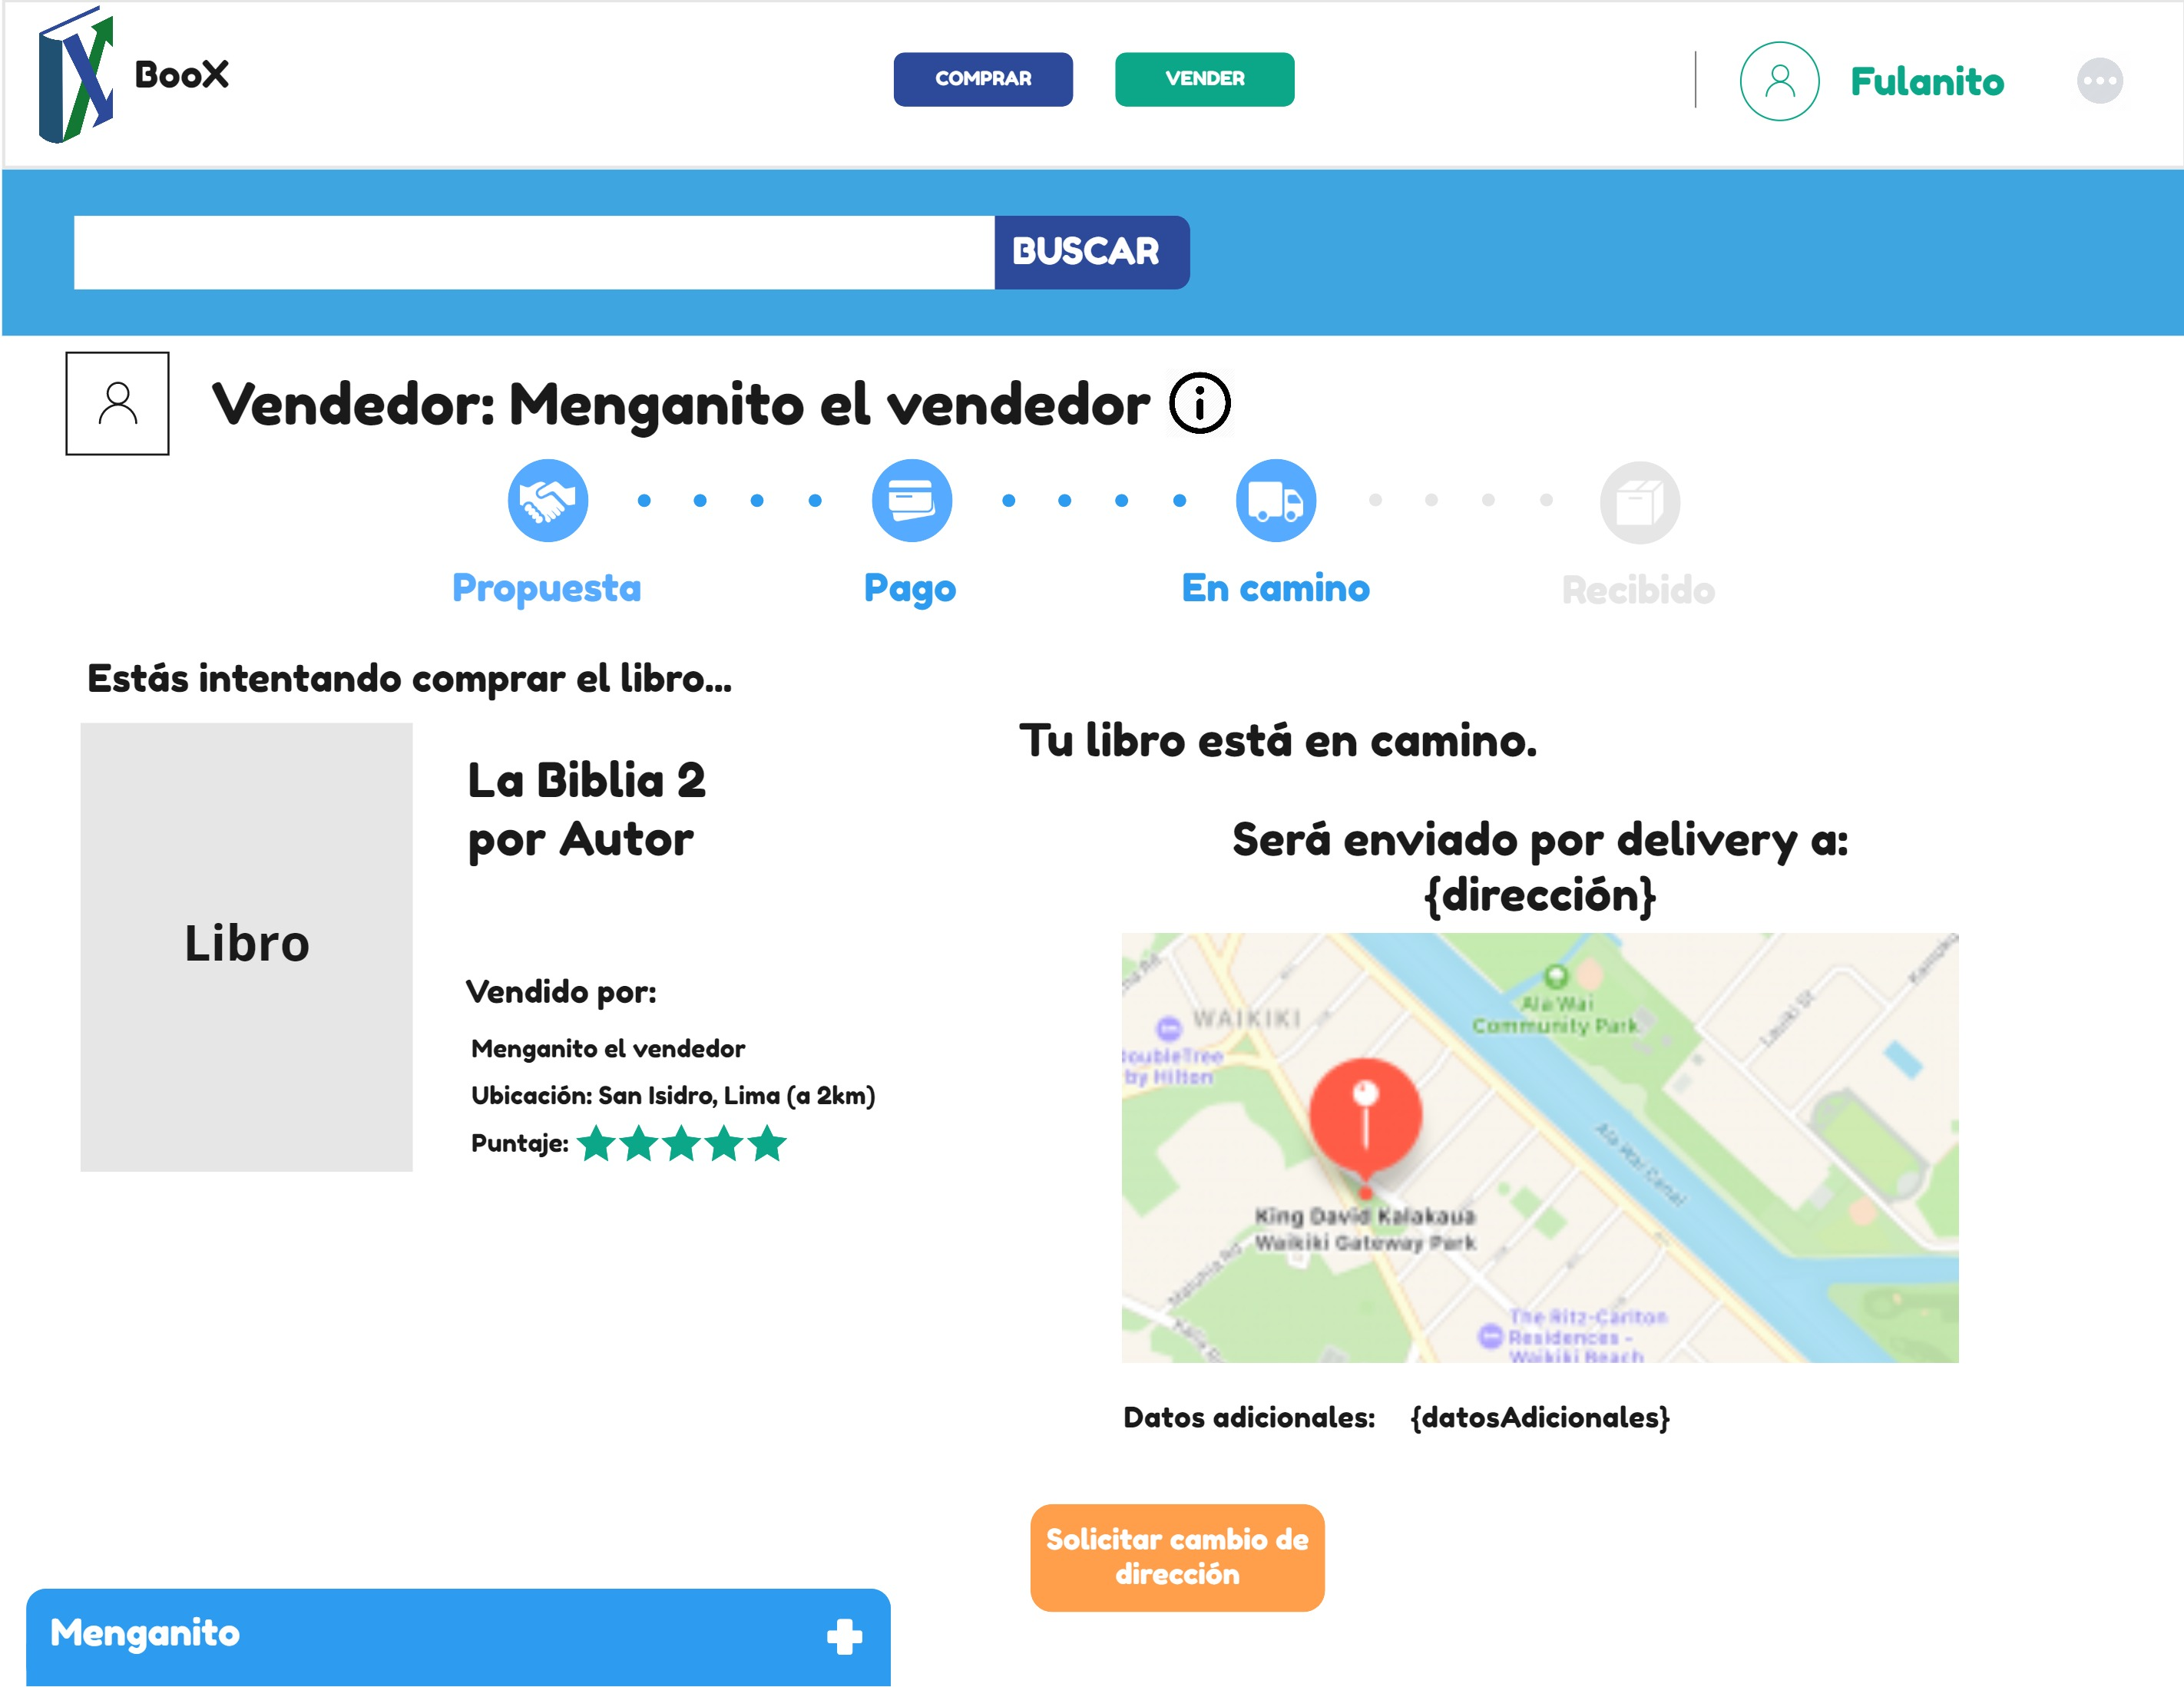
\includegraphics[width=300pt]{img/mockups/Huascar Retrieval Team - Contactar vendedor - En camino.jpg}
    \end{center}
    \subsubsection*{}
    \begin{center}
    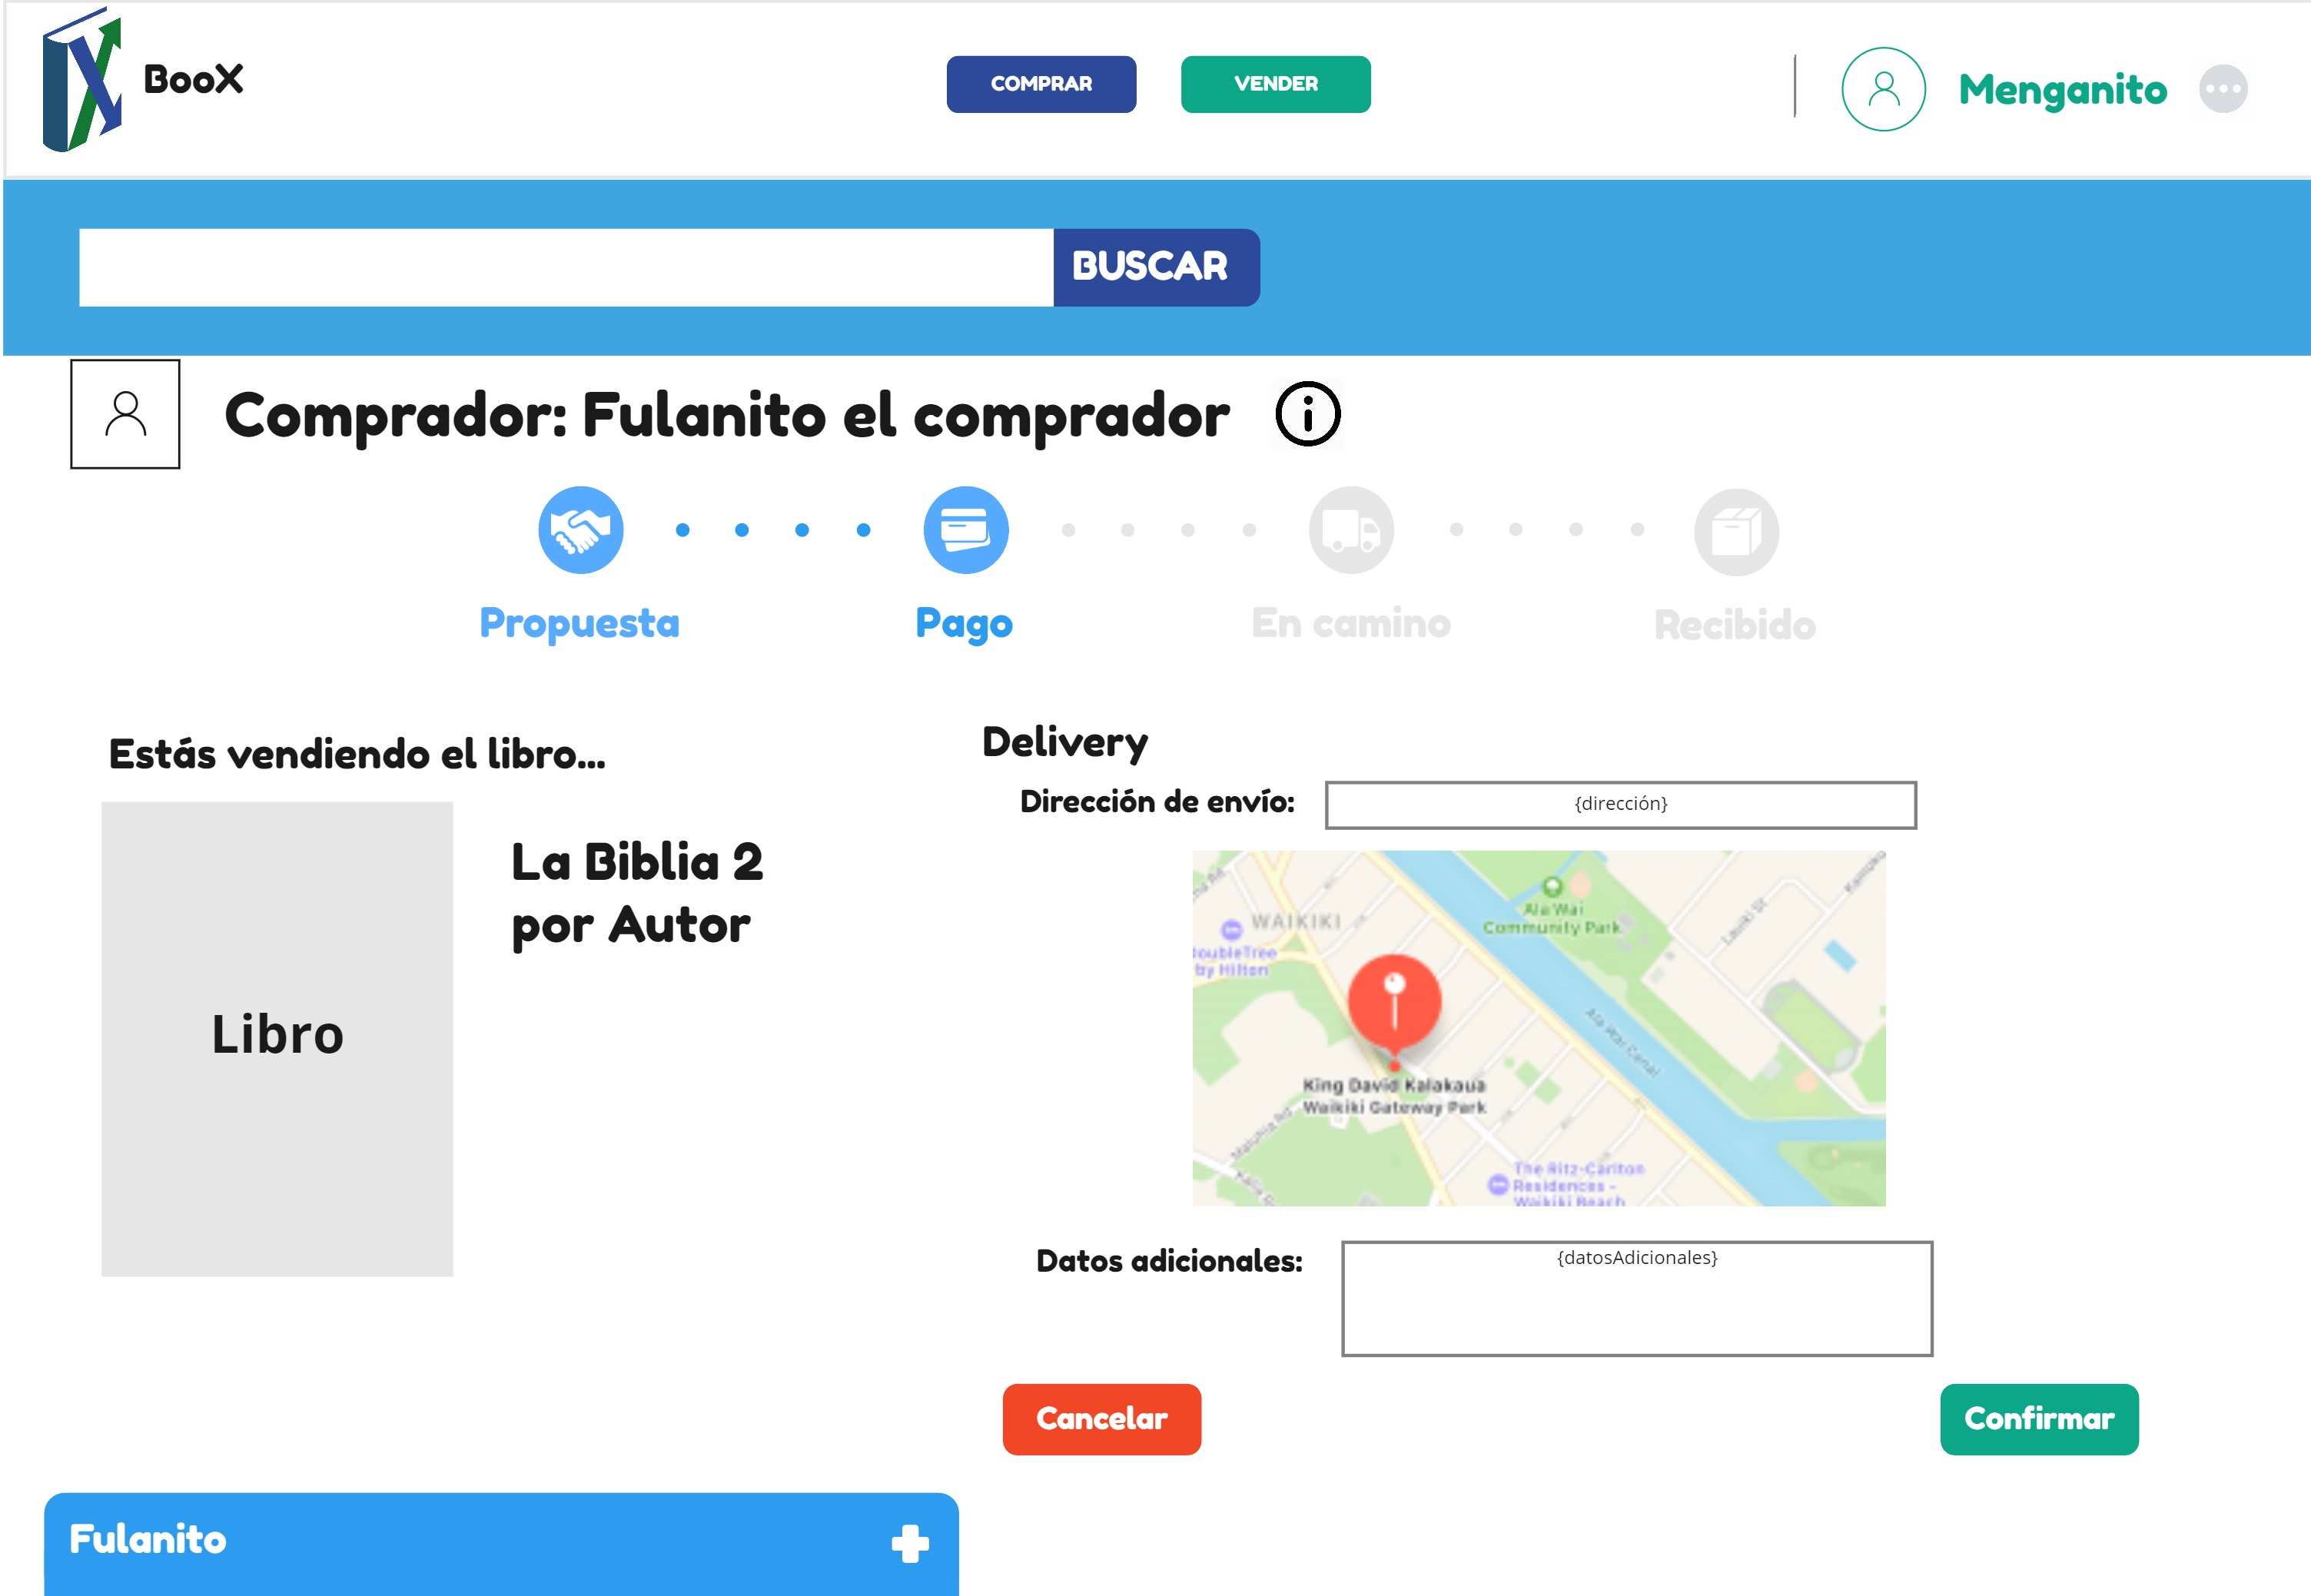
\includegraphics[width=300pt]{img/mockups/Huascar Retrieval Team - Vendedor siendo contactado (4).jpg}
\end{center}


Before sending the book, both the seller and buyer have the "cancel" option. Because this is a destructive action, the following pop up is presented when trying to cancel. The same logic applies when the buyer cancels.
\begin{center}
    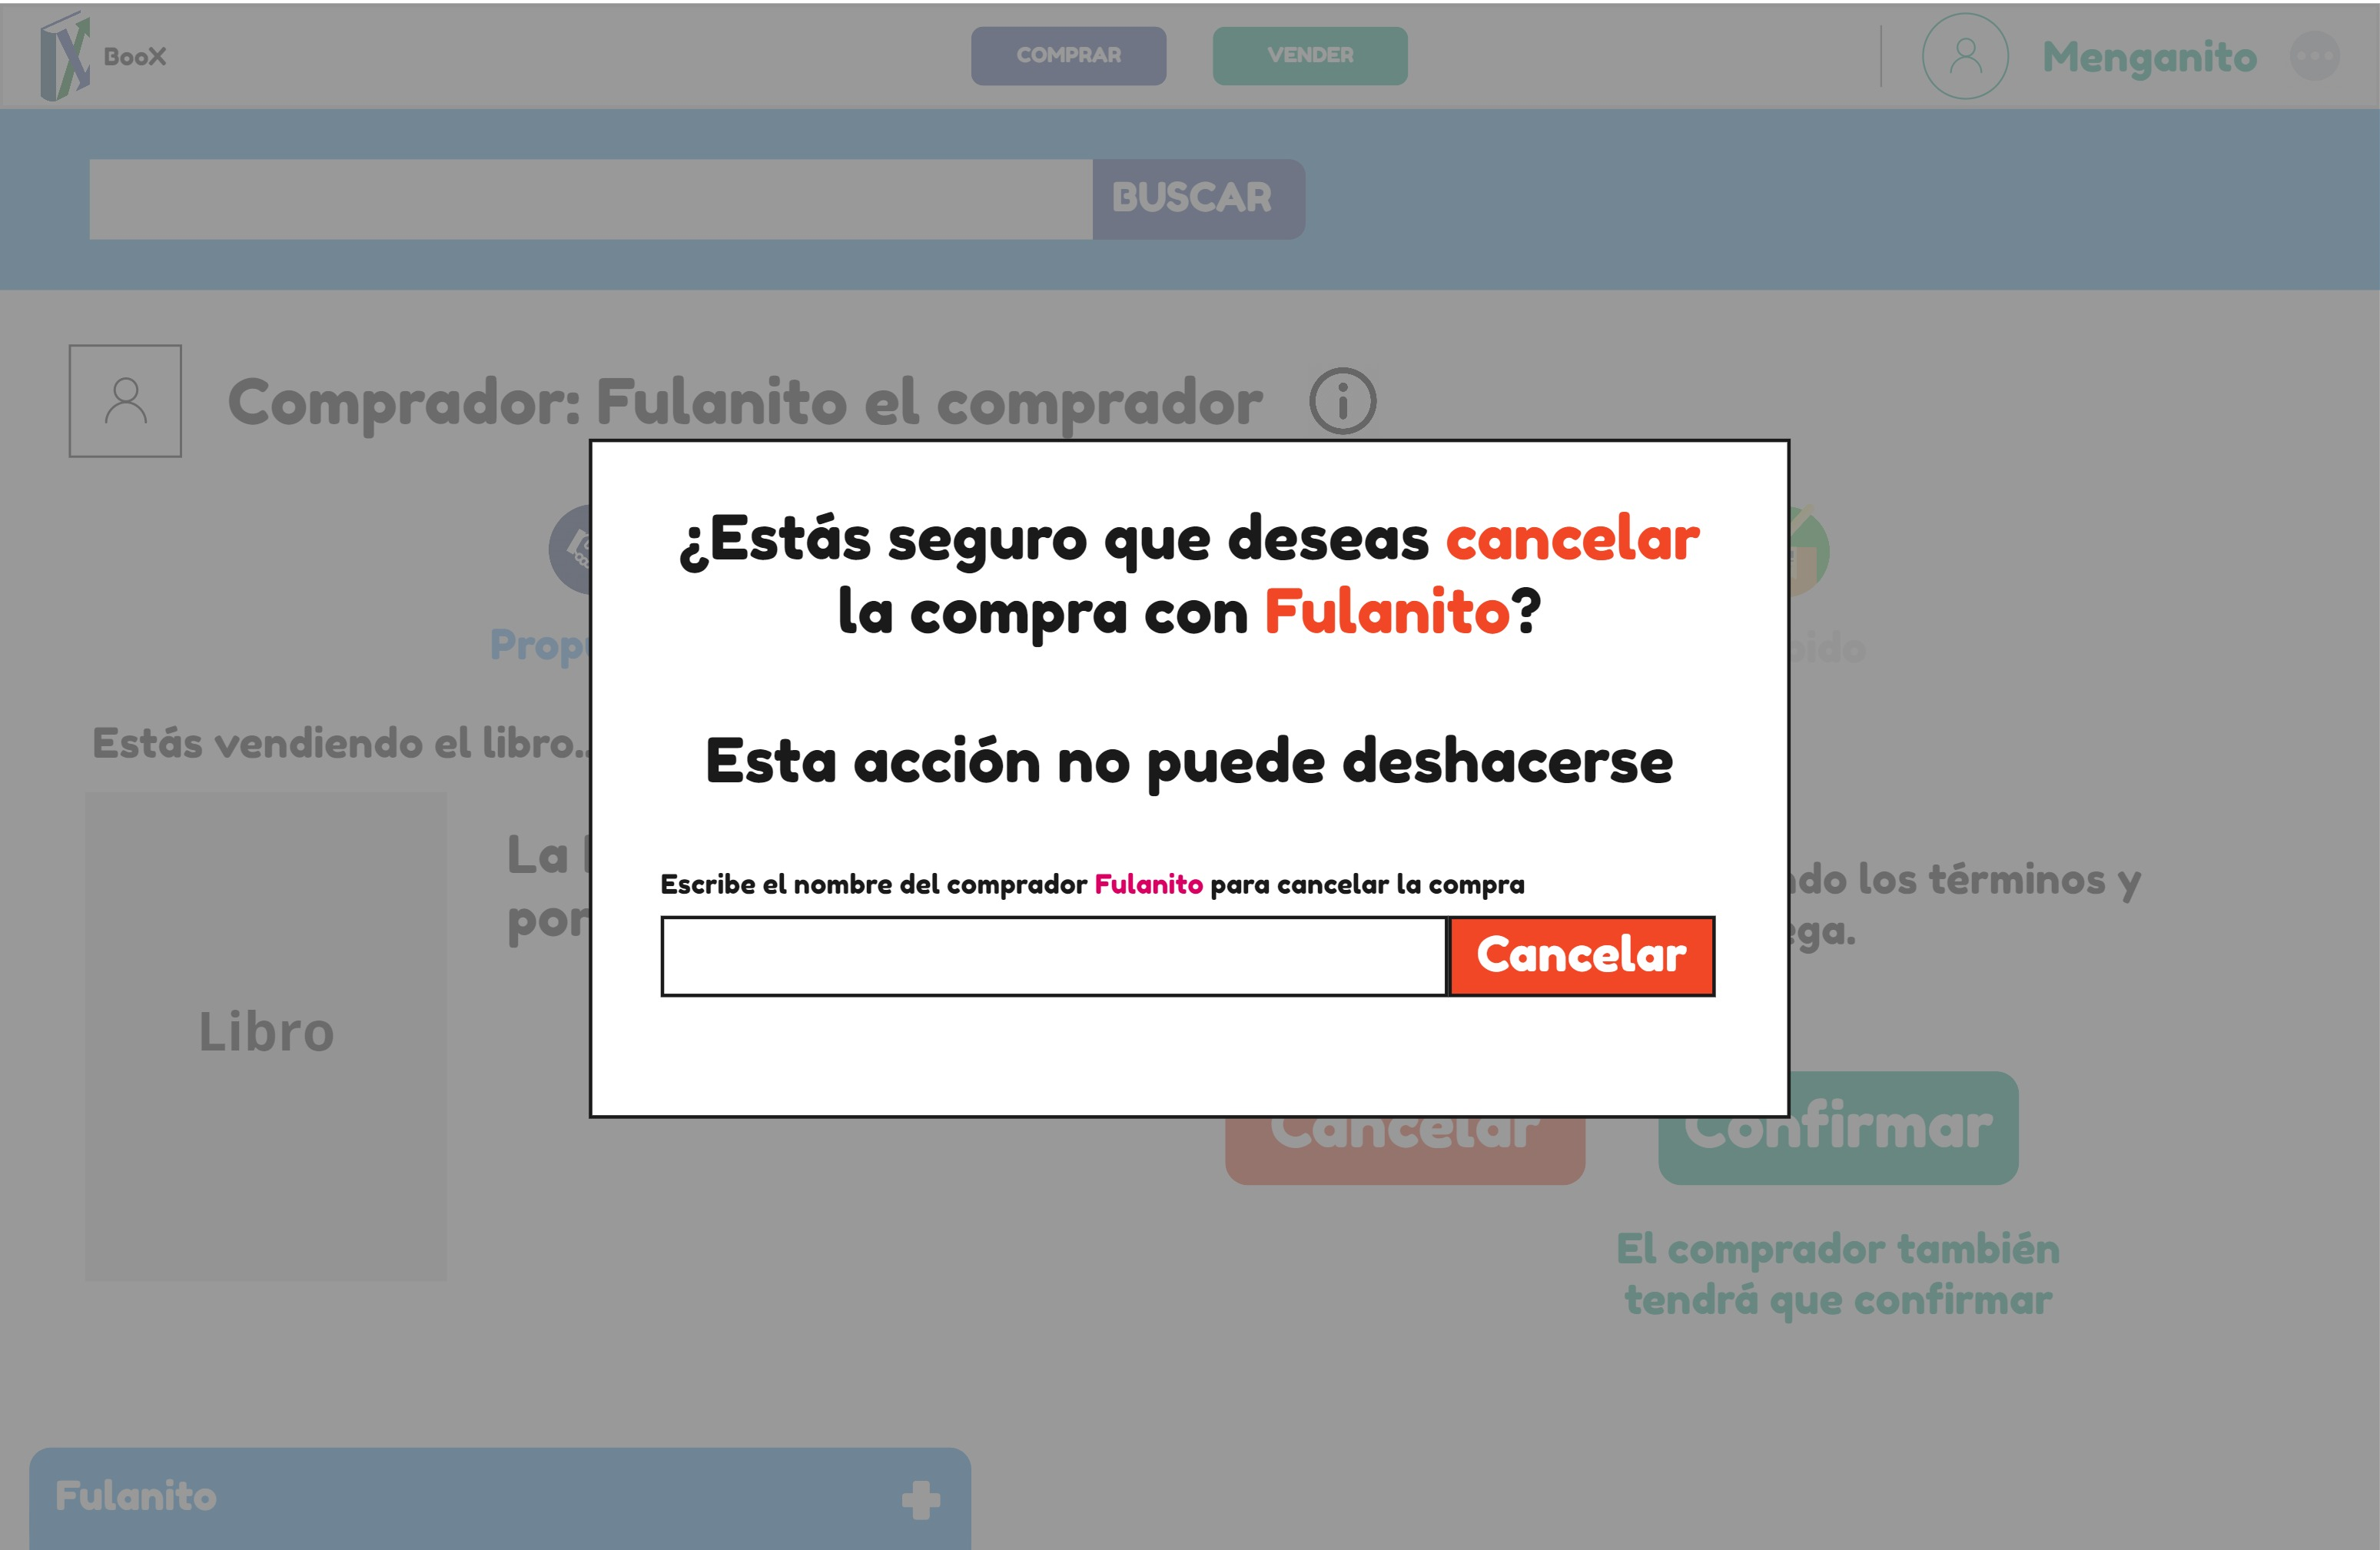
\includegraphics[width=300pt]{img/mockups/Huascar Retrieval Team - Vendedor siendo contactado (2).jpg}
\end{center}